user\chapter{Trabalhos Relacionados}

\section{Introdução}

Escrever sobre trabalhos relacionados

\section{Augmented Reality}
\subsection{Innovative Real-time Navigation Assistance to Wheelchair Users}
The  RT navigation assistance mobile application was developed by Abdalla et al. \cite{abdallah2019} to afford wheelchair users with motor disabilities mobility assistance, which consists of guiding them from a source point to a desired destination. 

Based on the user needs, the authors developed the Augmented Reality System for the Assistance of Wheelchair People (ARSAWP), which gives an augmented touch to accessibility information as presented by Figure \ref{fig:abdallah2019}. It also allows for remote monitoring capabilities of such users. 

\begin{figure}[!hbt]
\begin{center}
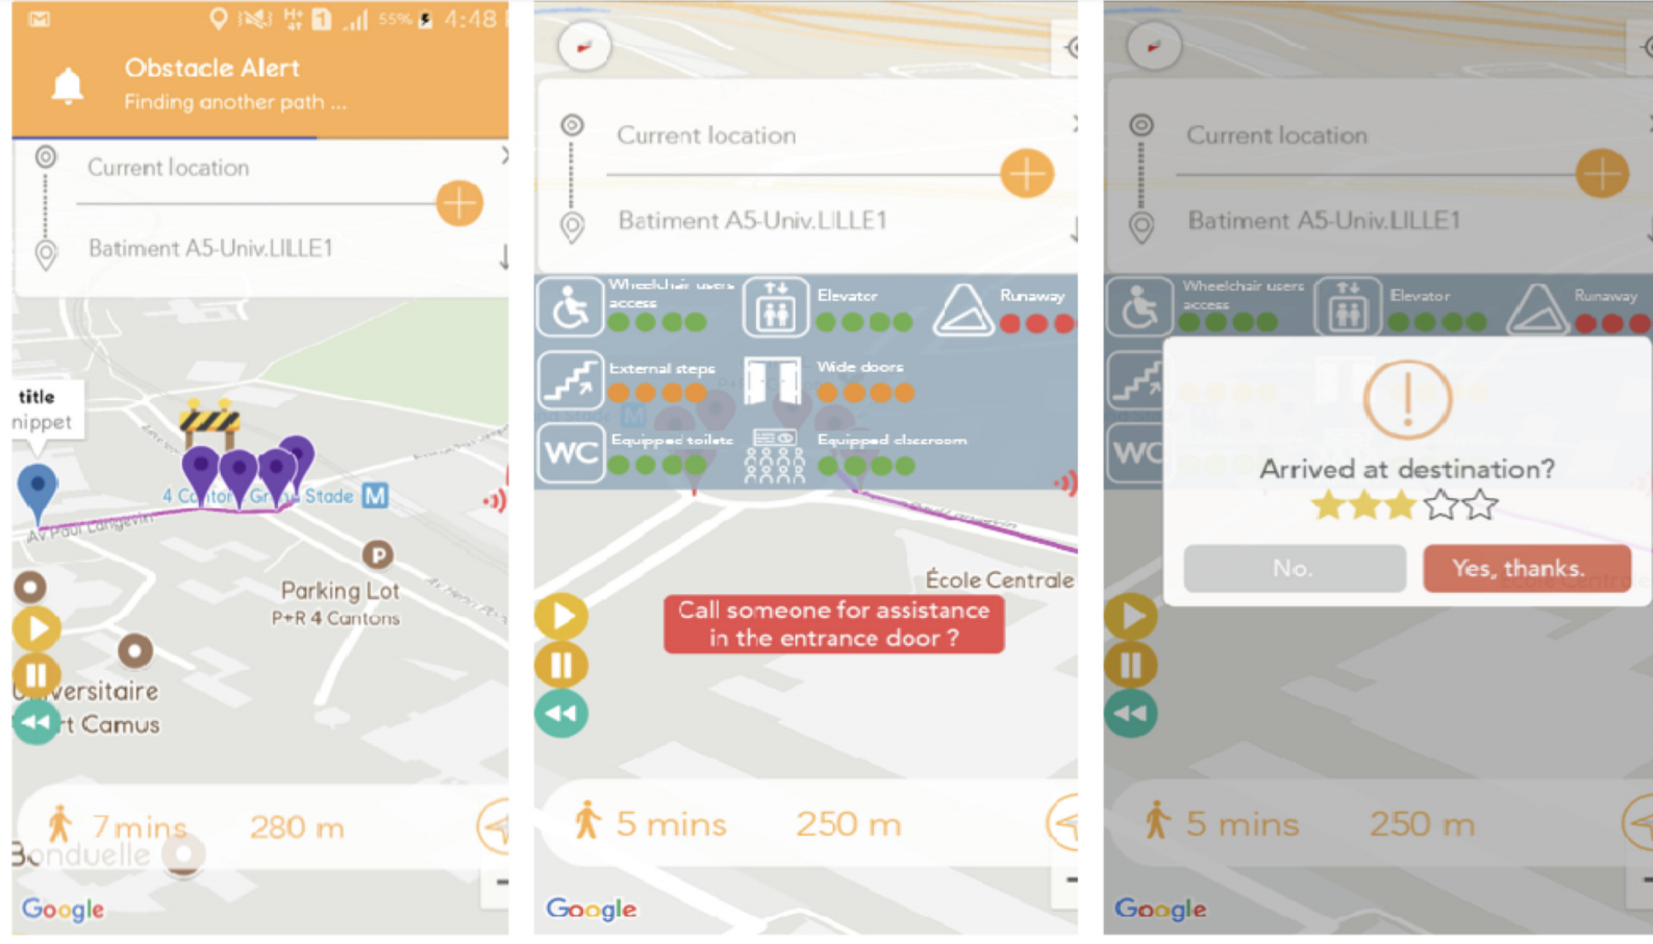
\includegraphics[width=0.9 \textwidth]{img/cap3/abdallah2019}
\caption{Navigation system interfaces preview \cite{abdallah2019}}
\label{fig:abdallah2019}
\end{center}
\end{figure}


The ARSAWP gives them a glimpse of accessibility information concerning the desired destination whether it is accessible, accessible with assistance or not accessible at all, according to his current location. After the user has chosen their destination, the ARSAWP creates a RT accessibility graph based on the user’s Global Positioning System (GPS) coordinates and the area cartography supported by an innovative Dijkstra algorithm. The ARSAWP notify the user when an obstacle is detected on the way. Then, the ARSAWP reroutes to another obstacle-free path. Obstacles already reported by other users are included in the obstacles management system to notify wheelchair users the presence of potential obstacles. ARSAWP handles a real-time display of obstacles and paths on a map using Google Maps Application Programming Interface (API).

In this case, it is observed that the AR techniques are useful by guiding the wheelchair user, improving the activities of daily living. This technique increases the user's traveling journey due to virtual information visualized. Features like these can be exciting in the process of training of PW users.

\subsection{Head-Mounted for Explainable Robotic Wheelchair Assistance}

Robotic wheelchairs controls have been improving with a wide range of unconventional input methods, such as brain-machine interfaces and head motion. Also, improvements in navigational assistance algorithms have contributed to bettering user technology integration for powered mobility, as opposed to traditional joystick control. The lack of sensorimotor capacity to steadily navigate an environment, using a standard joystick-controlled wheelchair, had shown up the necessity to engage shared control.

Although these features are added to ensure user safety, they may disorient or frustrate the user hindering user’s ability to learn how to navigate a wheelchair and thus leading to their failure to acquire ownership of these mobility platforms. The AR HMDs have recently gained attention as training simulators for off-line learning of wheelchair control. However, AR HMDs can potentially serve as a more transparent mode of communicating assistance, but still have to be integrated into physical wheelchairs for on-line operation. 

Based on the difficulty that severely disabled individuals present to build a mental model of their robotic wheelchairs behavior under different environmental conditions, Zolotas et al. \cite{zolotas2018} proposed this work as shown in Figure \ref{fig:zolotas2018}.

\begin{figure}[!hbt]
\begin{center}
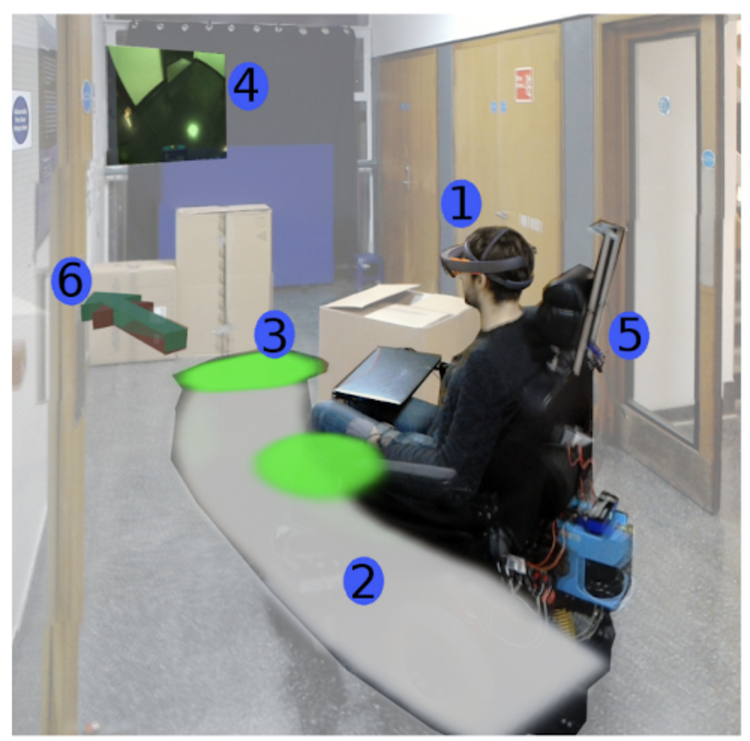
\includegraphics[width=0.7 \textwidth]{img/cap3/zolotas2018}
\caption{Hololens AR system \cite{zolotas2018}}
\label{fig:zolotas2018}
\end{center}
\end{figure}

Where: 
\begin{enumerate}
\item Composite image of the visualisations rendered on the
user’s view through the AR headset;
\item The grey path shows the trajectory generated by the user’s manual input;
\item The green patches highlight objects that pose as potential collisions;
\item The rear view display captures;
\item The camera image mounted on the back of the seat which includes overlaid graphics, such as the path and obstacle cues; and
\item The green and red directional arrows represent the user’s raw input and the corrected output, respectively.
\end{enumerate}

To explore the assistive effects of AR on wheelchair control, 16 non-disabled participants in where they were invited to complete a navigation route four times, in sequence.
The author's findings show the integration of AR HMDs with robotic wheelchairs, brings benefits. For instance, the rear-view display yielded enthusiastic participant responses by presenting helpful information to users at a comfortable and non-intrusive viewing angle, as long as certain design choices are taken into account.

The Microsoft Hololens was used in this case as an immersive way to augment the user experience and to highlight the benefits of AR techniques into the wheelchair users ADL. Nevertheless, the Microsoft Hololens is only capable of enriching the 3D real environment where the user is and not a remote one. It might represent a constraint, once many users are not able to address to a rehabilitation center and need telerehabilitation to support them to achieve it.

\subsection{Augmented Robotics for PW to Enhance Mobility}
A robotic framework able to plan and control a part of the route according to a normal HMI based on AR is proposed by Maule et al. \cite{maule2017}. 

Indeed, mobile robotics is an important discipline that provides autonomous systems from medicine to industrial applications to support humans' needs. AT like PW has a considerable impact on the quality of life of users affected in their mobility due to spinal cord injuries or degenerative diseases as Amyotrophic Lateral Sclerosis (ALS). Many of these users need a caregiver to help them in there ADL, but it doesn't improve their self-esteem. In order to improve their autonomy, different AT has been developed to reduce this feeling such as a joystick, keyboard, breath or eye tracker to control the PW. In most severe cases, as mention before, the users get very tired for being focused on the screen the whole time. Moreover, not all disabled people have the possibility to adapt their house increasing the challenges. 

The semi-autonomous HMI developed with AR techniques to control the PW  brings great benefits to relieve the user during difficult maneuvers.  The proposed AR-based application presented in Figure \ref{fig:maule2017}, is able to recognize points of interest (POIs) presented and recognised by fiduciary AR markers from the Kinetic V2.0. 

\begin{figure}[!hbt]
\begin{center}
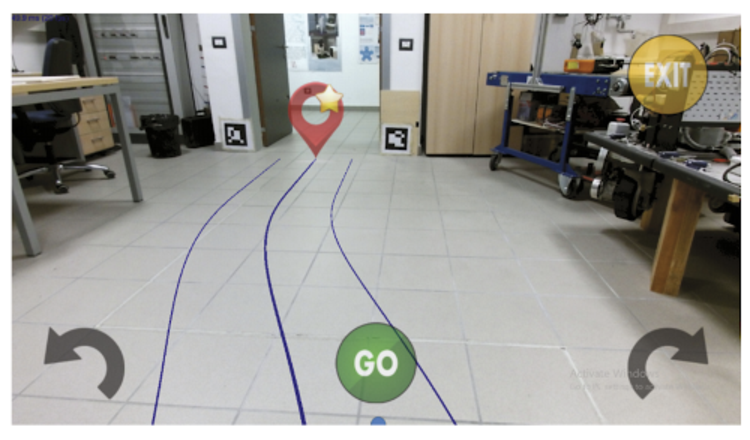
\includegraphics[width=0.94 \textwidth]{img/cap3/maule2017-AR}
\caption{HMI for the control of the wheelchair \cite{maule2017}}
\label{fig:maule2017}
\end{center}
\end{figure}

When a POI enters in the field of view of the camera, the user can select it by his/her eye movement captured by TOBII EyeX (eye tracker). To start the semi-autonomous maneuver, the user must explicitly select the POI by gazing it for 3 seconds. 

Based on the semi-autonomous system's main features, the authors realize some future issues to be implemented from the preliminaries tests. The AR techniques used to increase the user's experience during their activities doesn't present any failure based on Kinect V2.0 used as a camera. However,  they realized the need to implement an on-line calibration process to Kinect before start using the  system to reduce the position failures during the long periods of use. 

Among the various characteristics, AR takes advantage of all the information in the real world and uses it to benefit the enrichment of the user experience. With the rendering of virtual objects on the fiducial markers, the user can interact with the existing POIs with their eyes.  By activating the semi-automatic system to reduce their efforts or to control the PW through the options displayed on the screen. The HMI used in this work can in the future be incorporated into user training systems for PW and, with the use of telerehabilitation techniques, he can do distance training through a AR semi-immersive, using a monitor.

\section{PW Training}
\label{sec:pwTraining}
\subsection{Multisensory PW Simulator for Training and Rehabilitation}
A multi-sensory PW Simulator (PWS)  platform that provides visual, auditory and haptic feedback, as well as motion cues, is presented by Vailland et al. \cite{vailland2019}. Adaptive features of the framework allow integration with HMD, immersive rooms, single screens and the integration of add-ons and configuration adjustments to meet the individual needs of users. The authors aim to provide a realistic wheelchair driving experience for training and skill transfer to real-life situations.

The framework requirements were defined based on challenges lived for people experiencing mobility in where the PW driving is a challenging task that requires good visual, cognitive and visuospatial abilities. Occupational Therapists (OT), physiotherapists and neurologists analyzed the suggestion form filled out by the users from the Pole Saint Helier Physical Medicine and Rehabilitation Center to better highlight the features \cite{vailland2019}.

Two  3D scenes (outdoor and indoor) were respectively reproduced based on ``Rennes Metropole''(Figure \ref{subfig:vailland2019-3dScenes01}) and ``Pole Saint Helier''(Figure \ref{subfig:vailland2019-3dScenes02}) using the widespread 3D engine Unity3D to visually render 3D scenes. VR techniques were chosen to better fit with the motion platform used to truly reproduce the kinematics and the controllers increasing the Sense of Presence (SoP). 

\begin{figure}[!h]
\center
\begin{minipage}{0.495\linewidth}
\center
\captionsetup{justification=centering,margin=0.5cm,font=small}
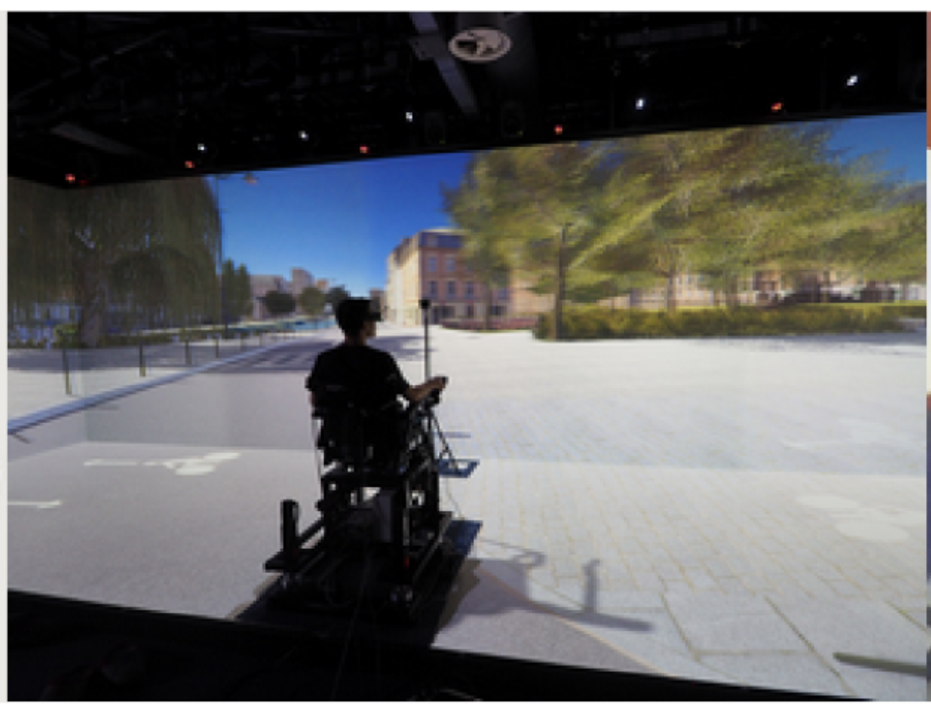
\includegraphics[width=0.95\linewidth]{img/cap3/vailland2019-3dScenes01}
\caption{ Outdoor scene \cite{vailland2019}} \label{subfig:vailland2019-3dScenes01}
\end{minipage}
\begin{minipage}{0.495\linewidth}
\center
\captionsetup{justification=centering,margin=0cm,font=small}
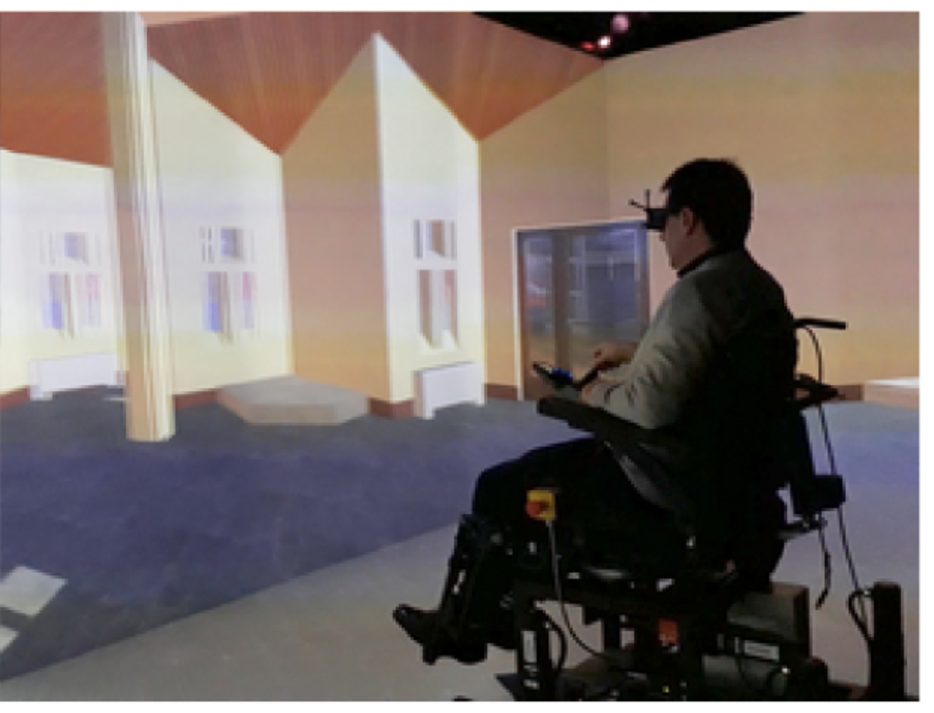
\includegraphics[width=0.95\linewidth]{img/cap3/vailland2019-3dScenes02}
\caption{ Indoor scene \cite{vailland2019}} \label{subfig:vailland2019-3dScenes02}
\end{minipage}
\end{figure}

The integration tests were performed and the authors considered the current issues to be addressed futurely, such as:
\begin{itemize} 
\item Setup limitations regarding motion feedback to control all 4 DoF and to enhance the simulator kinematics in order to handle interactions with the environment such as bumps, vibrations and collisions; and
\item The Virtual Environment (VE) to provide visual feedback and also to populate 3D scenes with dynamic entities such as avatars, vehicles, etc.
\end{itemize}

Further, the clinical assessment with PW users to evaluate the impact of the various feedback modalities provided by the simulator on SoP and cybersickness has to be assessed.

Although VR is widely used in simulators, it is not easy to adjust the platform implantation to increase the user SoP. On the other hand, in an augmented controlled room with real physical objects, static and animated virtual objects, a therapist can fit individuals protocols better. Thus, the user is able to have a natural and realistic training process and using telerehabilitation techniques he/she doesn't need to move to a rehabilitation center. 


\subsection{Protocol for driving a PW using RV}
\label{sec:valentiniPMRT2019}
The Unified Health System and the centers are responsible for the concession and dispensing services of AT equipment, such as, for example, the PW.

For this, one must consider some eligibility criteria for PW prescription and training, in order to guarantee the safety and autonomy of the AT user, to avoid the abandonment of the equipment and their exposure to accidents during their ADL. In fact, during these activities, there are unforeseen situations that require specific maneuvers in the PW, limiting their social participation and the recovery of their independence.

VR its being used widely in many different situations in medicine areas for training purposes in past years \cite{vailland2019,john2018, kamaraj2016, mahajan2013}. For this reason, Valentini et al. \cite{valentini2019} present a comparative study, split into two groups. One performs first in a VE (Figure \ref{fig:valentini2019virtual}) with audible warnings for each task accomplished and then the real protocols scenery (Figure \ref{fig:valentini2019real}). The other carries out a set of protocols in real scenery.

\begin{figure}[!hbt]
\begin{center}
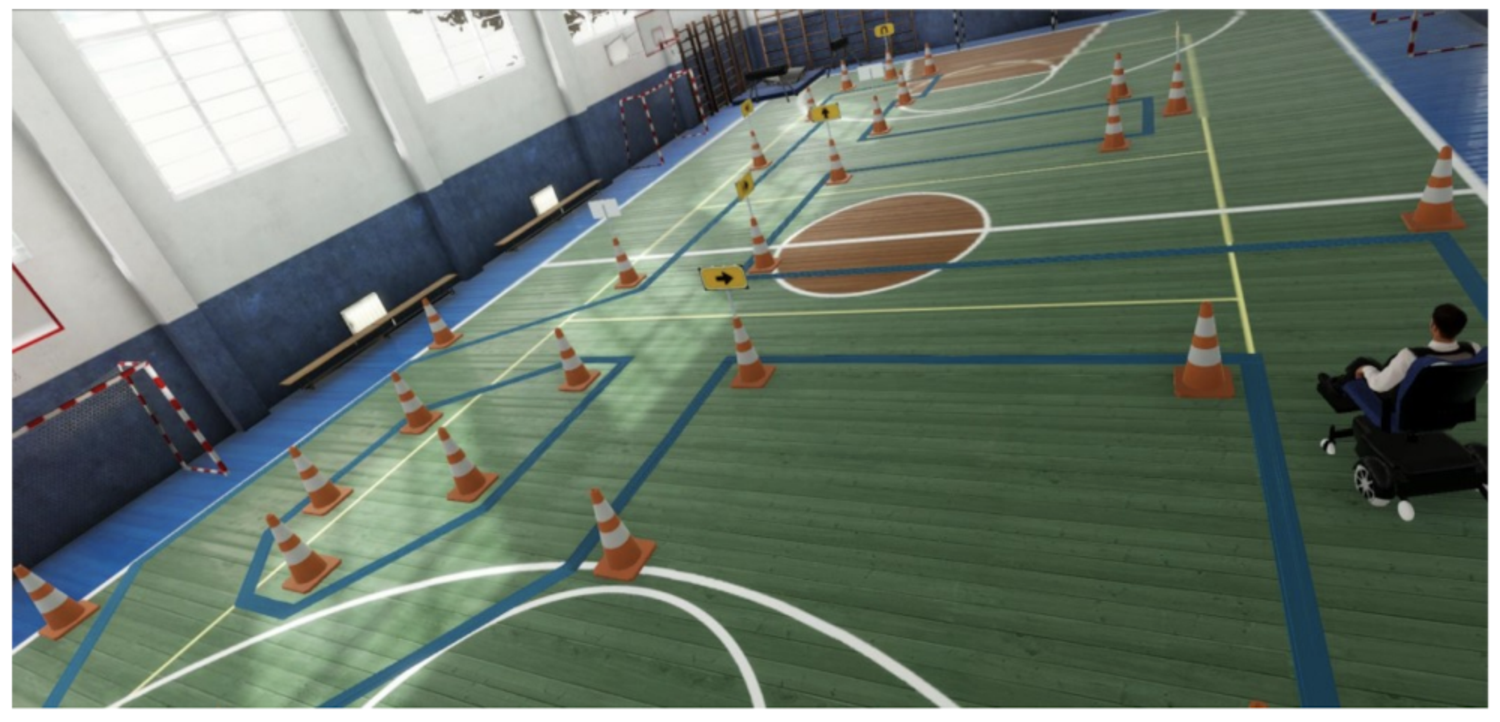
\includegraphics[width=1 \textwidth]{img/cap3/valentini2019virtual}
\caption{VR intervention training \cite{valentini2019}}
\label{fig:valentini2019virtual}
\end{center}
\end{figure}

\begin{figure}[!hbt]
\begin{center}
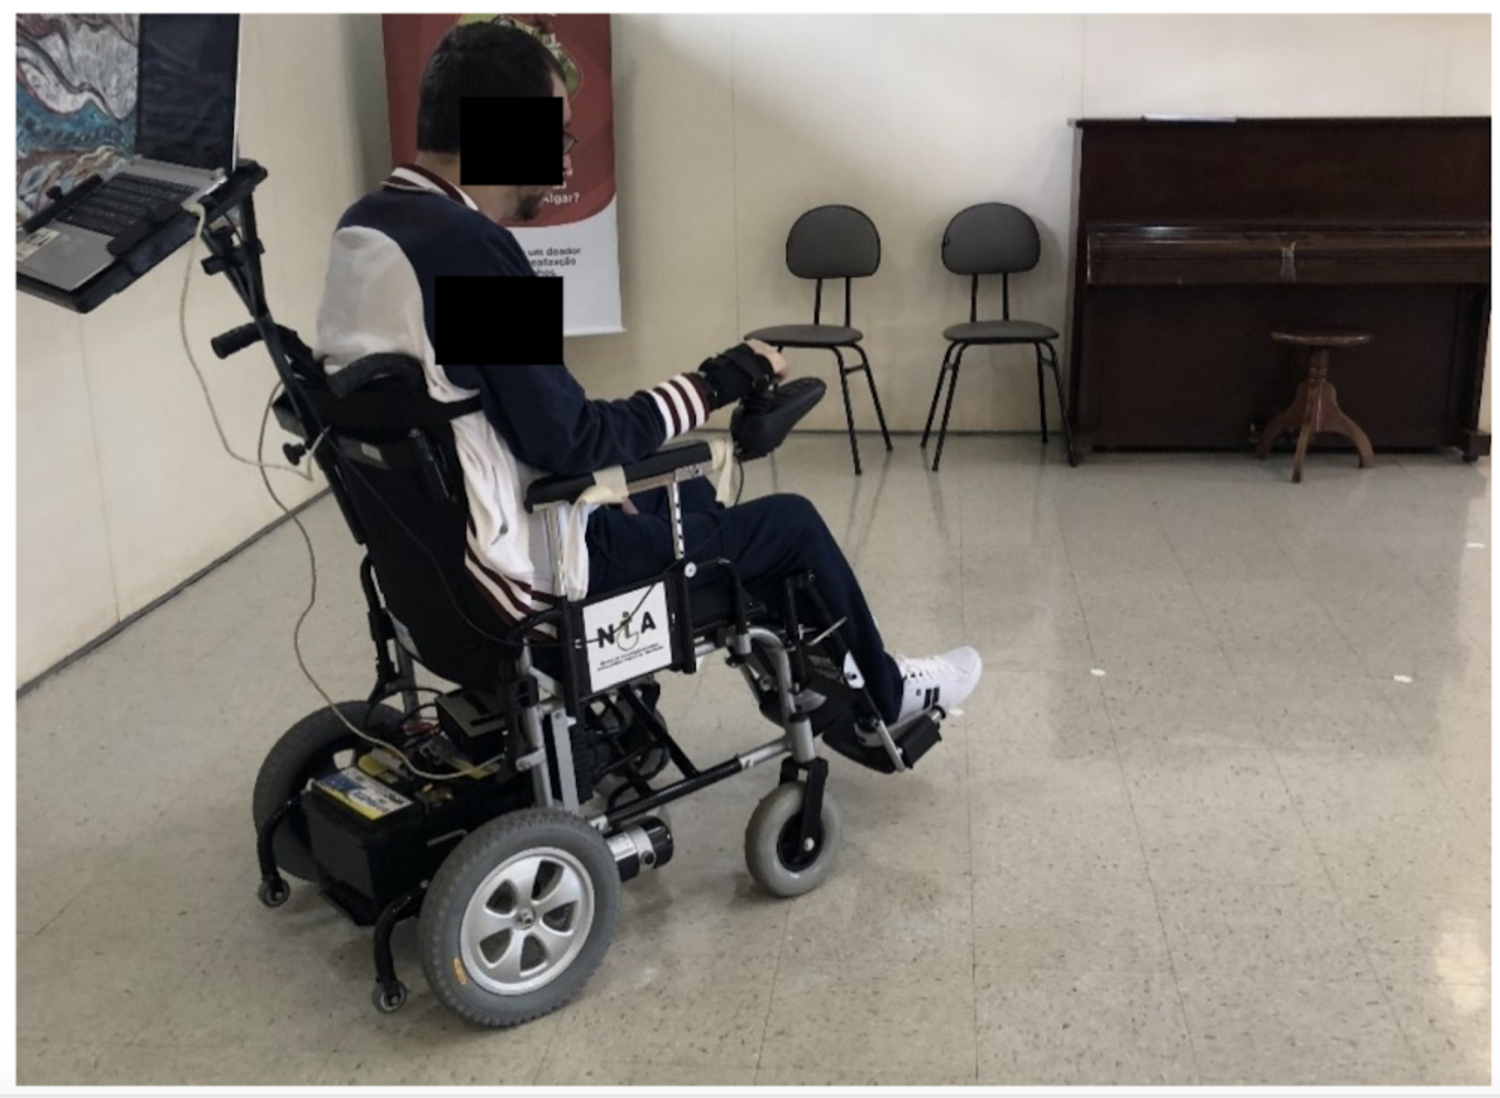
\includegraphics[width=0.8 \textwidth]{img/cap3/valentini2019real}
\caption{Real intervention training \cite{valentini2019}}
\label{fig:valentini2019real}
\end{center}
\end{figure}

The study carried out brought up many considerations, such as:

\begin{itemize}
\item The users who underwent VR through intervention showed better development in the execution of the tasks in comparison to the real interventions;
\item Users reported difficulties in using the simulator, as they felt lost during the performance of each set of tasks, despite the sound signals as the activities were completed;
\item Others considered it strange to perform activities on a sports court;
\item It was not possible to meet the needs of each user individually; and
\item Users reported that the design of some scenarios should be improved, suggesting clues with better realism, with objects and obstacles better distributed.
\end{itemize}

Based on considerations made by users, it is noticeable that VR environments still have limitations, such as non-adaptive scenarios and ineffective realism. All of these limitations could easily be addressed using AR techniques. The protocols could be defined in real-time, through the previous selection of the animated or static virtual objects that would compose a series of tasks and also, use arrows to guide the user during the tasks.

Finally, the use of telerehabilitation techniques and distributed systems would make the user experience even easier, since he could remotely connect to the system by performing the actions proposed remotely by the therapist.

\subsection{Virtual Environment for Training PW Manoeuvres}
Learning the necessary driving skills can be a daunting task, particularly for individuals with severe, or multiple motor limitations \cite{rodriguez2015}. 

Despite VR has been utilized in various training scenarios, previous research appoints that price and technology limitations have been a barrier to commercial adoption.  In contrast, affordable, high fidelity interfaces for VR such as the Oculus Rift HMD are now becoming readily available. 

Based on these facts, John et al. \cite{john2018} present a more intuitive, immersive VE for training users of PW that can easily be deployed and in which a new user of a PW
can quickly learn how to operate it. 

The authors do not attempt to reproduce reality, rather they use abstract tasks.  Figure \ref{fig:john2018task-a} present on the left: go through doorway and on right: traverse a circle and reach out to press a light switch. Figure \ref{fig:john2018task-b} shown on the left: slalom and on the right: reverse parking. These components task helps to develop the same skills required and used during PW navigation.

\begin{figure}[!htbp]
\center
\begin{minipage}{0.5\linewidth}
\center
\captionsetup{justification=centering,margin=0.5cm,font=small}
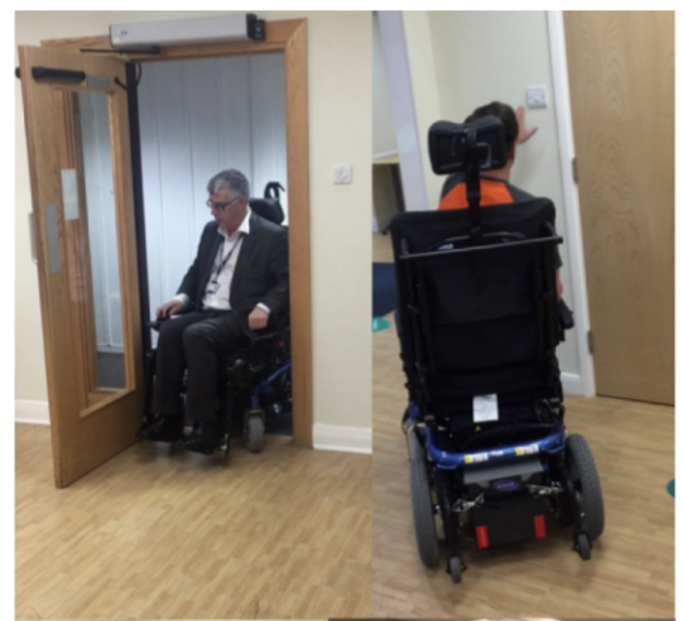
\includegraphics[width=0.93\linewidth]{img/cap3/john2018task-a}
\caption{Task components (a) \cite{john2018}} \label{fig:john2018task-a}
\end{minipage}
\begin{minipage}{0.492\linewidth}
\center
\captionsetup{justification=centering,margin=0cm,font=small}
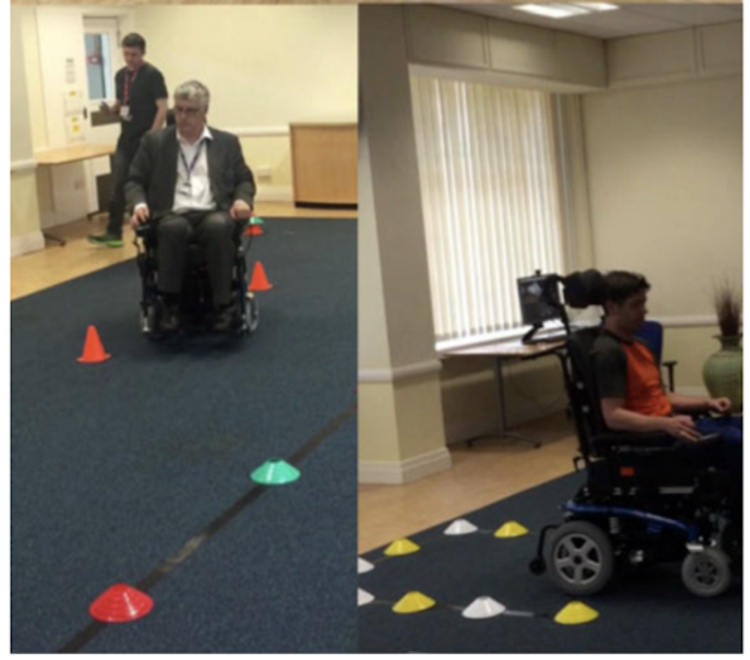
\includegraphics[width=0.95\linewidth]{img/cap3/john2018task-b}
\caption{Task components (b) \cite{john2018}} \label{fig:john2018task-b}
\end{minipage}
\end{figure}

For the first test, thirty-three able-bodied volunteers were randomly divided into three groups of eleven: 
\begin{itemize}
\item A Control group who would receive no training; 
\item A group wearing the ``HMD'' (Figure \ref{fig:john2018virtual}) having an immersive experience with PW-VR application; and
\item A ``Desktop'' group who also uses  PW-VR, but just with a desktop monitor having a semi-immerse experience, as presented by Figure \ref{fig:john2018virtual}.
\end{itemize}

\begin{figure}[!hbt]
\begin{center}
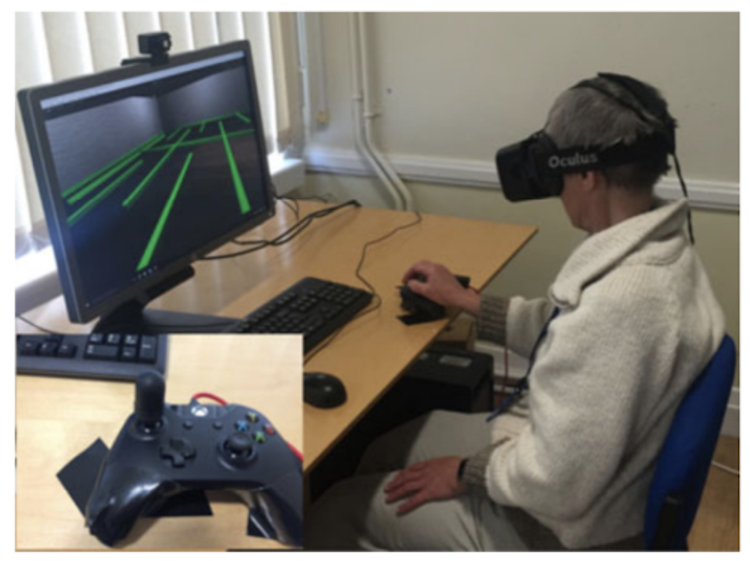
\includegraphics[width=0.95 \textwidth]{img/cap3/john2018virtual}
\caption{VR training environment \cite{john2018}}
\label{fig:john2018virtual}
\end{center}
\end{figure}

From the experiments performed the authors realizes: 
\begin{itemize}
\item The learning acquired in the HMD-based VR environment was transferred to the physical world; and 
\item There is a benefit in using a VR-HMD simulator for training wheelchair users, in terms of navigation performance improvement. 
\end{itemize}

However,  results from the SSQ (Simulator Sickness Questionnaire) indicate that cybersickness, the mismatch between physical and virtual motion in PW-VR for the HMD group, is a problem, even with a relatively short training session \cite{kennedy1993}.

The main focus of this work is to assess whether driving a PW skill increasing through an VR environment, using a HMD. As reported by the authors, no real volunteers were invited and it was not yet the focus of the work to assess the real challenges experienced by users. However, depending on the level of limitation of eligible users, not everyone will be able to use HMD and there is also the cybersickness effect that can be solved using AR techniques. Adapting tasks in VR environments to the needs of real users is still a challenge. In addition, these users may have to go to a rehabilitation center. In this way, the use of telerehabilitation techniques may allow the sharing of the environment between therapists and users through the Internet, reducing this need.

\section{Training assessment}
\label{sec:trainingassess}
\subsection{Protocol for driving a PW using VR}
Looking for best practices concerning training methodology and assessment tools, Valentini et al. \cite{valentini2019} studied the works proposed by \cite{john2018,martins2017,nunnerley2017, torkia2015,mahajan2013}.

John et al. \ cite {john 2018} presents the statistical training results between each of the groups of healthy participants through a one-way Analysis Of Variance (ANOVA). Nunnerley et al. \cite{nunnerley2017} have developed an immersive VR training system to build driving skills to eligible participants. Among them are, clinicians and experts PW users with Spine Cord Injury (SCI). Only the VE features were assessed. Due to limitations found, such as nausea and lack of VE realism that leads to minor training adherence, participants' training evolution was not performed. Martins et al. \cite{martins2017} and Mahajan et al. \cite{mahajan2013} used the PMRT to assess users' performance as shown in Figure \ref {fig:martins2017}. Torkia et al. \cite{torkia2015} brings up qualitative information about PW users' perspective, which is very important when it is decided to developed some technological solution to these users.

\begin{figure}[!hbt]
\begin{center}
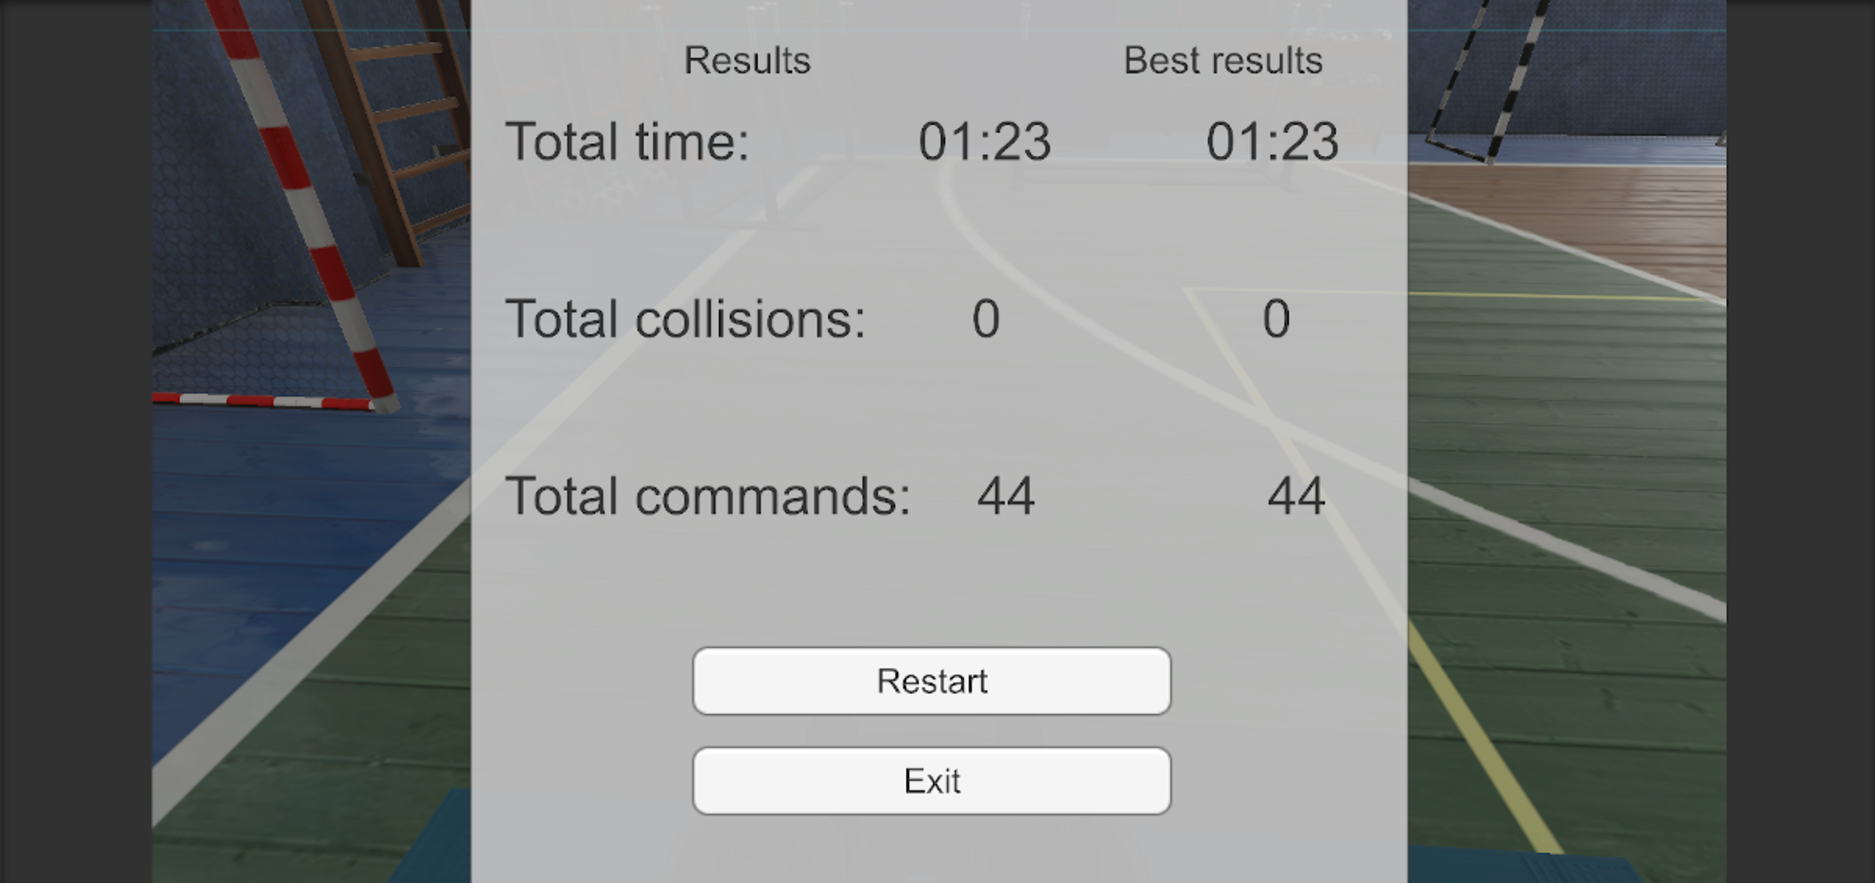
\includegraphics[width=1 \textwidth]{img/cap3/martins2017}
\caption{Results screen presented to the user \cite{martins2017}}
\label{fig:martins2017}
\end{center}
\end{figure}

Based on these previous work fundamentals, the authors have decided to use the PMRT, Power Mobility
IndoorDriving Assessment (PIDA) and the Power Mobility Community Driving Assessment (PCDA) to cover critical aspects of evaluation and activities present to the users \cite{dawson1994}. Some important feedback come from  \cite{valentini2019} research, like: 

\begin{itemize}
\item Many felt tired after the continuous execution of 12 of the 16 PMRT activities; and
\item The activities set was not individually fit to the participants.
\end{itemize}

Even applying an adaptation on PMRT, the users felt tired after the trials, and it was recognized, based on eligible participants, that not all of then were prepared to face some challenges established by PMRT. These observations have to be considered into the development of future training systems taking advantage of professionals' expertise to better fit individually training tasks and evaluate users' performance. Finally, Figure \ref{fig:martins2017} presents a metrics summary of the user performance at the trial moment. Nevertheless, the system offers the therapist an overall graphic of user metrics evolutions, which is very important to have an user evolution reading, across the trials.


\subsection{Virtual Environment for Training PW Manoeuvres}
John et al. \cite{john2018} present a more intuitive, immersive VR environment for training PW users, where the main focus is to prove that VR training intervention affords before real PW use.

ANOVA is applied to verify how significant the variance among the number of samples is.  So, applying it on a data set, it's possible to check which are the relevant training metrics, according to the participants' skills. 

The user evolution evaluation was obtained through the difference between each of the related metrics during each protocol performed. Such assessments come from the post-processing of the data collected. However, for an individual assessment, it's not desired and can not be accessed instantly using bar charts, that highlighting the participant's growth history. Comparative statistical analysis is essential for the scientific community, because it allows general analysis and cross-checking of information, but not from a single individual in a real-time telerehabilitation system.


\subsection{Improving individualized PW skills training satisfaction}
The World Health Organization identified that ``user training'' is a key requirement in the service delivery model of wheelchair provision \cite{who2008}. 

As a result, a lack of appropriate instruction leads to an ineffective use or even abandonment of wheelchairs and doesn't help the PW user who may struggle to use their mobile devices independently \cite{pettersson2014}. Tips and falls are the leading cause of injuries among PW users and it emphasizes the need for improved training opportunities to ensure that PW is used safely to their full capacity \cite{gaal1997,xiang2006}.

MacGillivray et al. \cite{macgillivray2018} work aims to test the hypothesis that PW mobility-related goal satisfaction improves following five Wheelchair Skills Training Program (WSTP) training sessions and improvements are retained 3 months post-training.

Seventeen PW users were submitted to five 30-min individualized, one-on-one, WSTP sessions at a targeted frequency of 1–2 sessions/week. Training occurred at the participant’s choice of location. Trainers helped participants to create PW mobility-related goals following  WSTP (version 4.1)  intervention and all goals set were required to have a mobility-related component \cite{kirby2008}.  Goals strictly based on wheelchair maintenance would not have been accepted.

Approximately, 5–10 goals were created over the course of the training. Upon setting each goal, participants in the current study were asked to report their goal satisfaction – ``how would you rate your current satisfaction with your ability to perform that goal on a scale from 0 to 10 with 0 being ‘not satisfied at all’ and 10 being ‘extremely satisfied’?'' \cite{mortenson2007}.  The one-way ANOVA was used to determine changes in the goal satisfaction scores.

The authors concluded that goal satisfaction following the WSTP improved years after initially learning how to operate a PW. The five training sessions were effective in improving goal satisfaction. A considered conclusion was that participants’ goal satisfaction scores were not significantly correlated with goal attainment scores recorded by the trainer, but mainly in meeting their needs.

It's not only the lack of technology quality applied to define a toolkit for PW users training that reduces the user adherence of the training, which leads to injury risk and TA abandonment. But meeting the PW user needs is an essential target in practice. Based on the clinical information and interview rises, the therapist knows how better guide this user through the driving skill improvement, enriching their well being and independence to realized their ADL activities. 

Thus, this study reinforces that to increase the adherence of any training process, to reduce AT abandon, it's essential to care about user's expectations, what they are prepared to do. For a telerehabilitation architecture that aims better-fit tasks by supporting PW user's training, adaptative features are mandatory.  


\subsection{Driver's stress detection using Skin Potential Response (SPR) signals}
\label{sec:stressSPR}
Car driving induced stress has a large impact on people’s wellness and can affect the way how they execute their activities. Being exposed to stress, can incurring car accidents \cite{zheng2015}.  The problem of automatic detection of car drivers’ stress levels has become increasingly important, due to its impact on people security, and more generally on people's health and well-being. 

Two approaches have been developed in order to detect stress: the first is based on physical measurements and the second is based on physiological measurements \cite{greene2016}. Among the various techniques proposed for stress detection, EDA monitoring is particularly interesting to gain information about the inner stress affecting a person, due to its correlation with the sympathetic nervous system response. 

Affanni et al. \cite{affanni2018}  propose a scheme based on EDA/SPR measurements show that, by appropriately processing EDA/SPR signals only, it is possible to efficiently locate stress events during driving. The authors propose an experimental setup, as shown in Figure \ref{fig:affanni2018} that allows defining a ground-truth for stress events recognition, and which confirms the validity of the proposed approach. 

\begin{figure}[!hbt]
\begin{center}
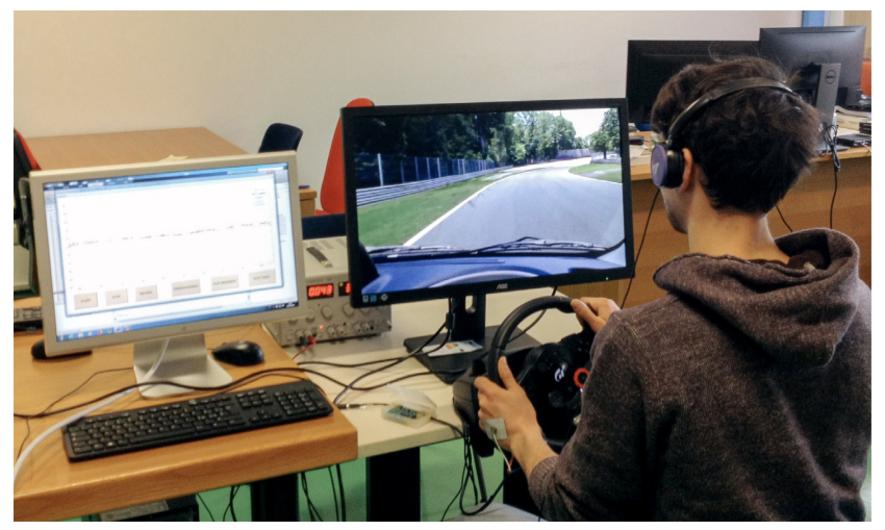
\includegraphics[width=1 \textwidth]{img/cap3/affani2018}
\caption{A picture of the test setup \cite{affanni2018}}
\label{fig:affanni2018}
\end{center}
\end{figure}

Tests were conducted in 15 subjects healthy conditions and with average driving experience. The experiments reveal it is effectively-identified stress triggers. The SPR signals can exhibit a complex behavior as noted by other authors,  which can make it challenging to associate peaks with stressing events unambiguously.

Toward a PW training system, it is important to defined a reliable assessment methodology to better evaluate the user evolves during the trials. However, without a biologicals measure like stress level, the therapist can not track possible emotional reasons for the user is not evolving or performing well in some tasks.  This approach brings a different look to the user's training towards their individualities, increasing the chances of success in enhancing their skills in driving the PW. 


\subsection{Interrater Reliability of the PMRT in the VR}
\label{sec:pmrtICC}
The injuries and accidents rate of PW users has increased in recent years, because the number of PW users also increased \cite{worobey2012}. This has intensified the need for better assessment and training programs for new PW users \cite{kirby2015}. The available driving assessment tools presented have clinicians with several obstacles, when assessing the ability to drive and train PW users to be time-intensive and non-standardized \cite{corfman2003}. It's hoped that driving simulators may meet this need for better assessment and training \cite{hogan2009}.

A Version 2 of the Virtual Reality-based Simulator (VRSIM-2) is presented by Kamaraj et at. \cite{kamaraj2016} to provide a safe environment, where new users can improve their PW driving skills. The main objective of the VRSIM-2 is to be an effective PW simulator in administering the PMRT  within a VE. In order to check this efficiency, a statistical analysis based on the clinician's or health professional score attributed to the PW user training tasks performed, called the Intraclass Correlation Coefficient (ICC), is used.  The ICCs values is interpreted as:  low (ICC<50\%), moderate (50\% - 75\%), and high (75\%).

To assess the ability of VRSIM-2 to achieve this goal, PMRT scores were used as a subjective measure of physicians' response and the Task Load Index developed by the National Aeronautics and Space Administration (NASA-TLX) was used as a subjective measure of users response as they interacted with different interfaces \cite{rubio2004}. Figures \ref{fig:kamaraj2016-InterfacesA}, \ref{fig:kamaraj2016-InterfacesB}, \ref{fig:kamaraj2016-InterfacesA} represents the environments first-person viewpoint training condition. The HMI existent are the customised joystick (Figure \ref{fig:kamaraj2016-InterfacesB}), encoders on rollers (Figure \ref{fig:kamaraj2016-InterfacesA}) and PW joystick. 

\begin{figure}[!htbp]
\center
\begin{minipage}{0.495\linewidth}
\center
\captionsetup{justification=centering,margin=0.5cm,font=small}
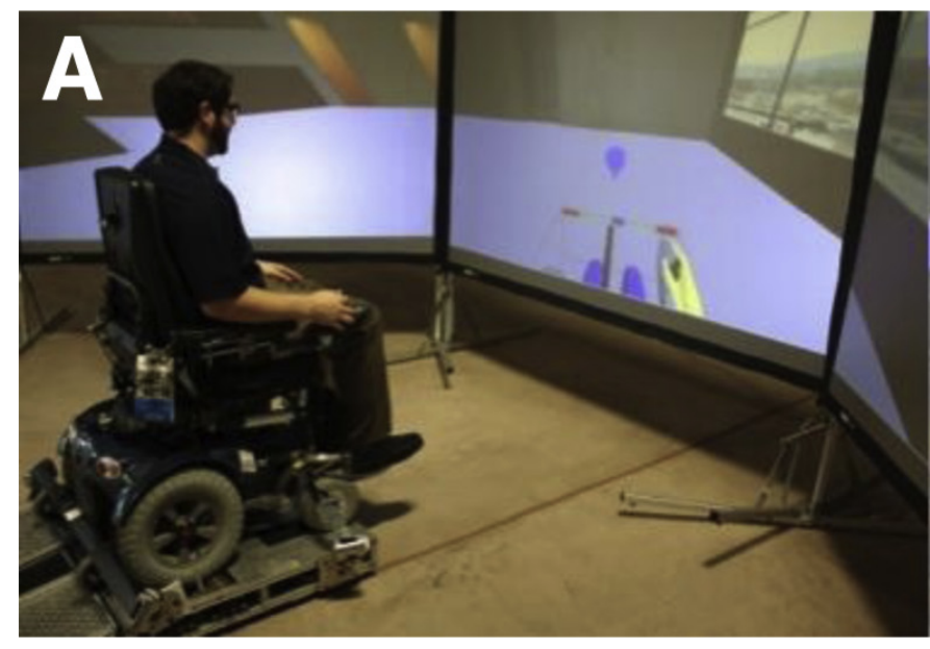
\includegraphics[width=1\linewidth]{img/cap3/kamaraj2016-InterfacesA}
\caption{VR display and rollers \cite{kamaraj2016}} \label{fig:kamaraj2016-InterfacesA}
\end{minipage}
\begin{minipage}{0.495\linewidth}
\center
\captionsetup{justification=centering,margin=0cm,font=small}
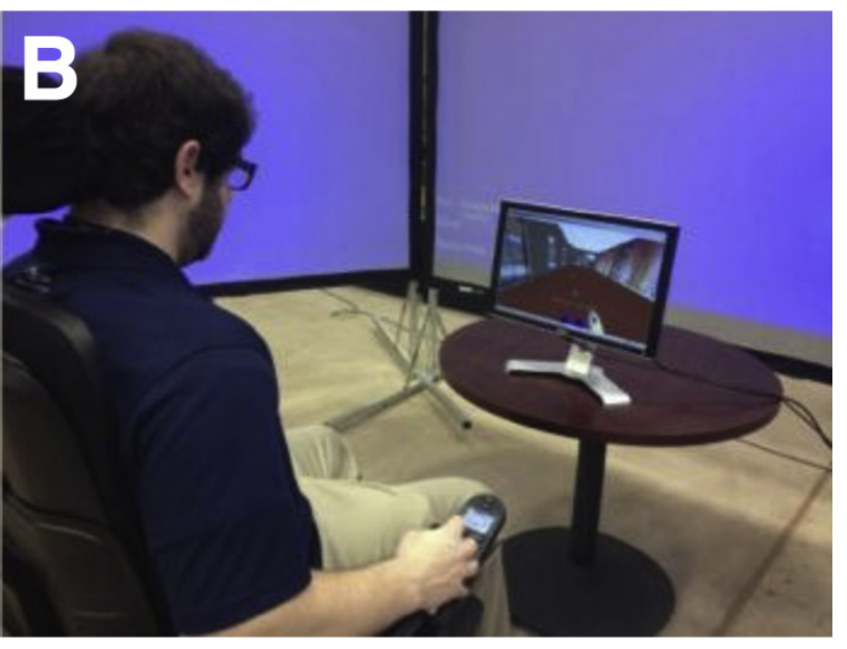
\includegraphics[width=0.92\linewidth]{img/cap3/kamaraj2016-InterfacesB}
\caption{Desktop VR screen and joystick interface \cite{kamaraj2016}} \label{fig:kamaraj2016-InterfacesB}
\end{minipage}
\begin{minipage}{0.495\linewidth}
\center
\captionsetup{justification=centering,margin=0.5cm,font=small}
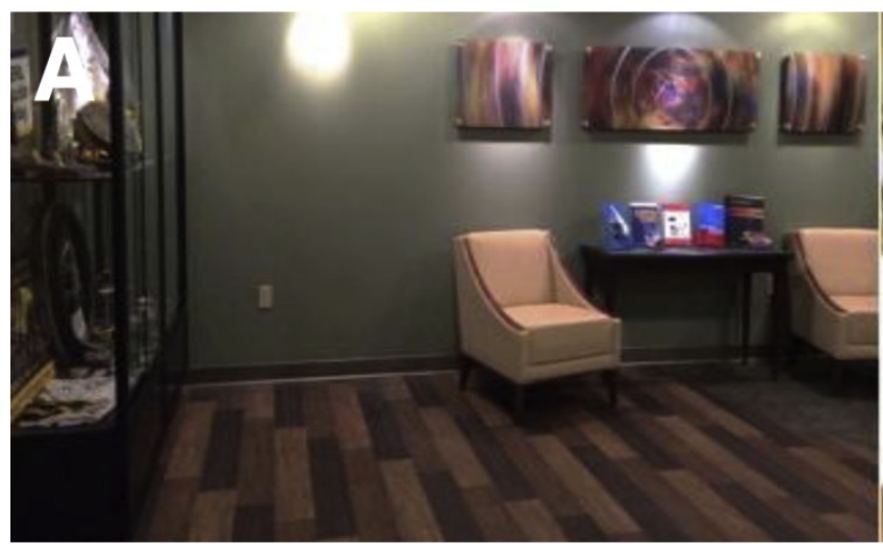
\includegraphics[width=1\linewidth]{img/cap3/kamaraj2016-VRA}
\caption{Real-world office lounge \cite{kamaraj2016}} \label{fig:kamaraj2016-VRA}
\end{minipage}
\end{figure}

Based on theses features, five different driving conditions were defined:
\begin{enumerate}
\item Desktop VR, rollers off and customised joystick interface controller;
\item Desktop VR, rollers on  and encoders on rollers interface controller;
\item VR display, rollers off and customised joystick interface controller;
\item VR display, rollers on  and encoders on rollers interface controller; and
\item Real-world scene, no rollers and PW joystick interface controller;
\end{enumerate}

Experiments were conducted in 21 PW athletes recruited from the 31st National Veterans Wheelchair Games where each one perform all conditions. From a group of 5 clinicians, 2 rates were randomly select to evaluate each participant.

The authors' results show that the PMRT had high interrater reliability between the two raters in all five driving conditions. Also, PMRT had a high interrater reliability in conditions 1 and 4 and could be used to assess PW driving performance virtually in VRSIM-2. 

Results present that the PMRT is a good methodology for the users' training assessment using a telerehabilitation system. Thus, different health professionals, even apart, may contribute equally with their results that can be used in the future for the scientific community based on a stable and reliable database.


\section{Telerehabilitation}
\subsection{AR Based Telerehabilitation System With Haptics (ARTESH) }
Borrosen et al. \cite{borresen2019} describes the features and utility of the system ARTESH which allows the sense of touch and direct physical musculoskeletal examination during a synchronous consultation. To reach an augmented experience presented by Figure \ref{fig:borresen2019}, the authors equipped each site with two Xbox Kinect, one haptic controller, a 3D-capable TV,  active 3D-glasses, and a computer. Thus, the 3D information collected by Xbox is rendered in real-time on 3D-glasses. 

\begin{figure}[!hbt]
\begin{center}
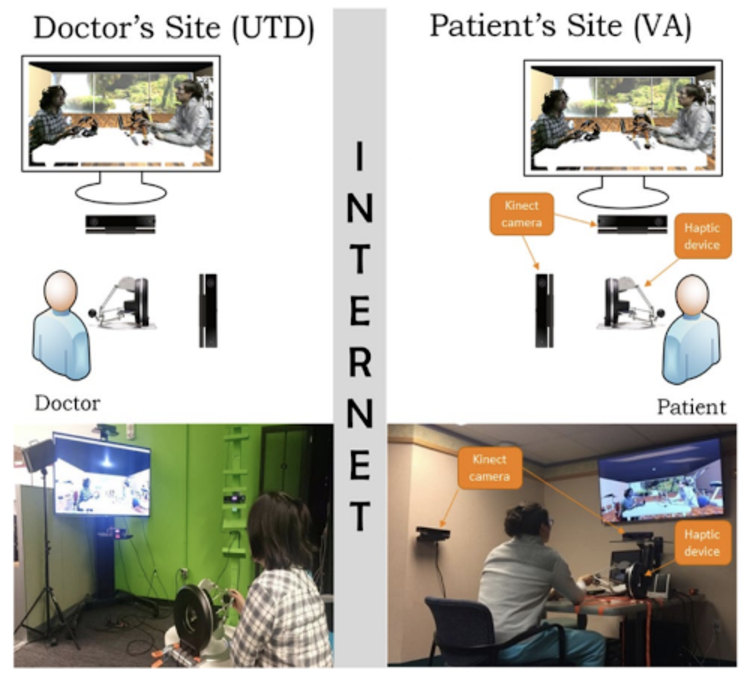
\includegraphics[width=0.6 \textwidth]{img/cap3/borresen2019}
\caption{Visual description of the setup at each site \cite{borresen2019}}
\label{fig:borresen2019}
\end{center}
\end{figure}

A pilot study with twenty volunteers evaluated the usability of the system \cite{schutte2012}. Among them, five healthy physicians and fifteen subjects referred to hospital-based PM\&R clinic with a chief complaint of the arm and/or shoulder pain or weakness, were recruited for the study.

Results suggest that the system was effective at conveying audio-visual and touch data in real-time across 20.3 miles and warrants further development. However,  the study’s findings may not be generalizable to all locations, because it requires ultra-high-speed Internet with high bandwidth and speed requirements.

In this study, AR was chosen as the base technology for the development of the teleworking system to allow a realistic real-time interaction between clinicians and users in safe conditions. Although, as the results point out, despite being accepted by users due to the feeling of presence, there is still a limitation in the quality of experience concerning real-time usage due to Internet quality restrictions.

Borrosen et al. \cite{borresen2019} demonstrated in this work that is possible to merge a Telerehabilitation experience with AR techniques. However, the authors result highlight that the Internet quality can reduce user feeling experience and notice the importance to be aware of bandwidth restrictions for telerehabilitation systems.



\subsection{Kinesiotherapy Device for Hands Rehabilitation}
\label{subsec:pani2014}

\cite{pani2014} present the development of a kinesiotherapy device applied to rheumatic users' rehabilitation. This device is presented in Figure \ref{fig:pani2014-device} and allows for remote monitoring capabilities of such users. In order to help recover their abilities, users are requested to execute an exercise protocol, for which all performance data are stored. Two main operation modes are available as:

\begin{figure}[!hbt]
\begin{center}
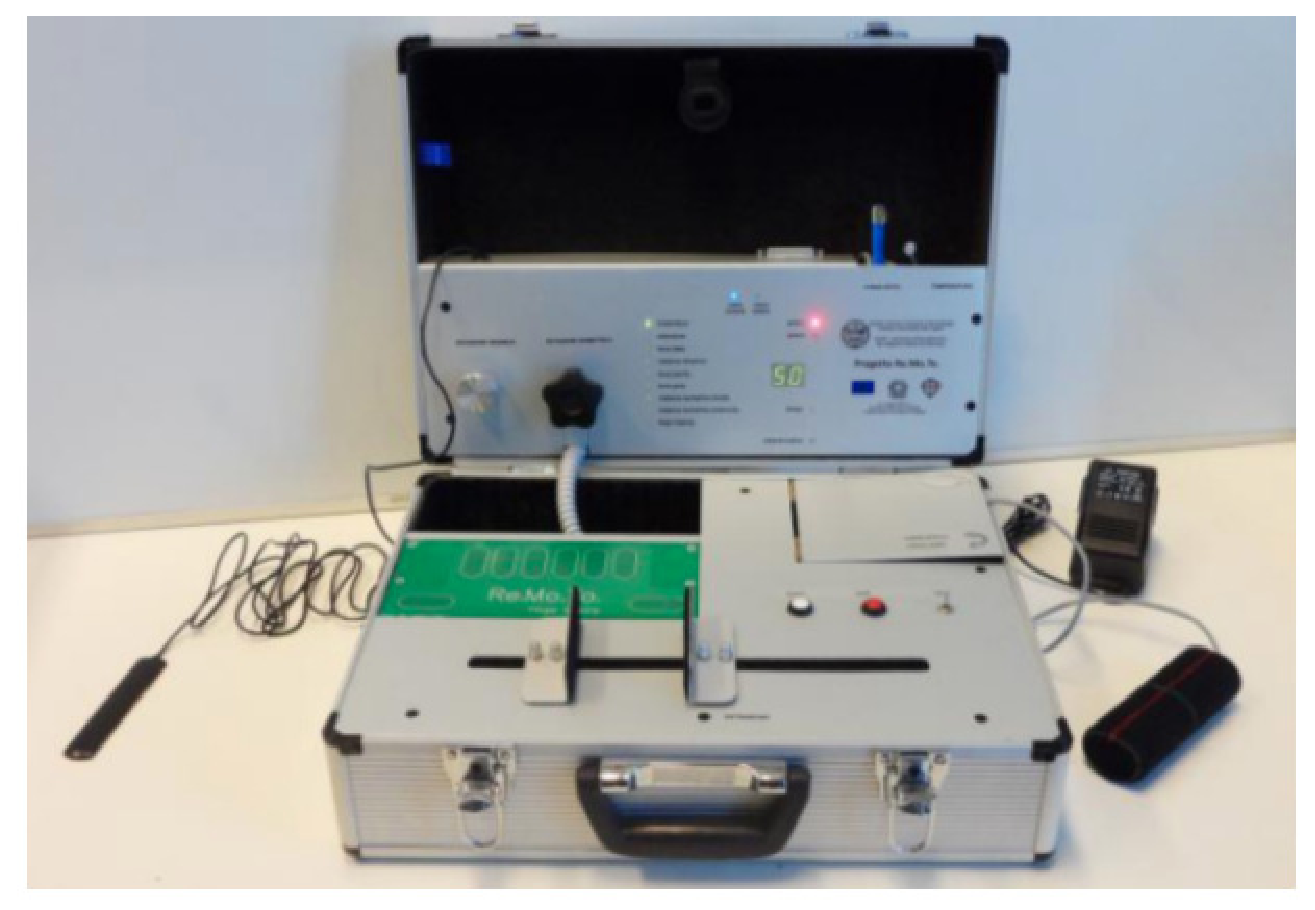
\includegraphics[width=0.7 \textwidth]{img/cap3/pani2014-device}
\caption{Proposed telerehabilitation device \cite{pani2014}}
\label{fig:pani2014-device}
\end{center}
\end{figure}

\begin{enumerate}[label=(\alph*)]
\item Real-time control mode: In this mode, users execute the proposed exercises under local supervision of a therapist; and
\item Deferred tele-monitoring mode: In this mode, the device guides the user through the execution of the exercises without local supervision. Performance data is sent to a remote server and will be available for further analysis by the therapist.
\end{enumerate}

On real-time control mode, the user executes a set of proposed exercises and a set of statistic data is sent to the therapists' computer, connected to the rehabilitation kit, via Bluetooth. On deferred tele-monitoring mode, after the proposed exercises' execution, statistic data is sent to a remote server, connected to the rehabilitation kit via Global System for Mobile  (GSM)/ General Packet Radio Service (GPRS) \cite{pani2014}. The therapist may then access this data on the remote server, using the Internet. Figure \ref{fig:pani2014-components} presents the main components of the proposed solution.

\begin{figure}[!hbt]
\begin{center}
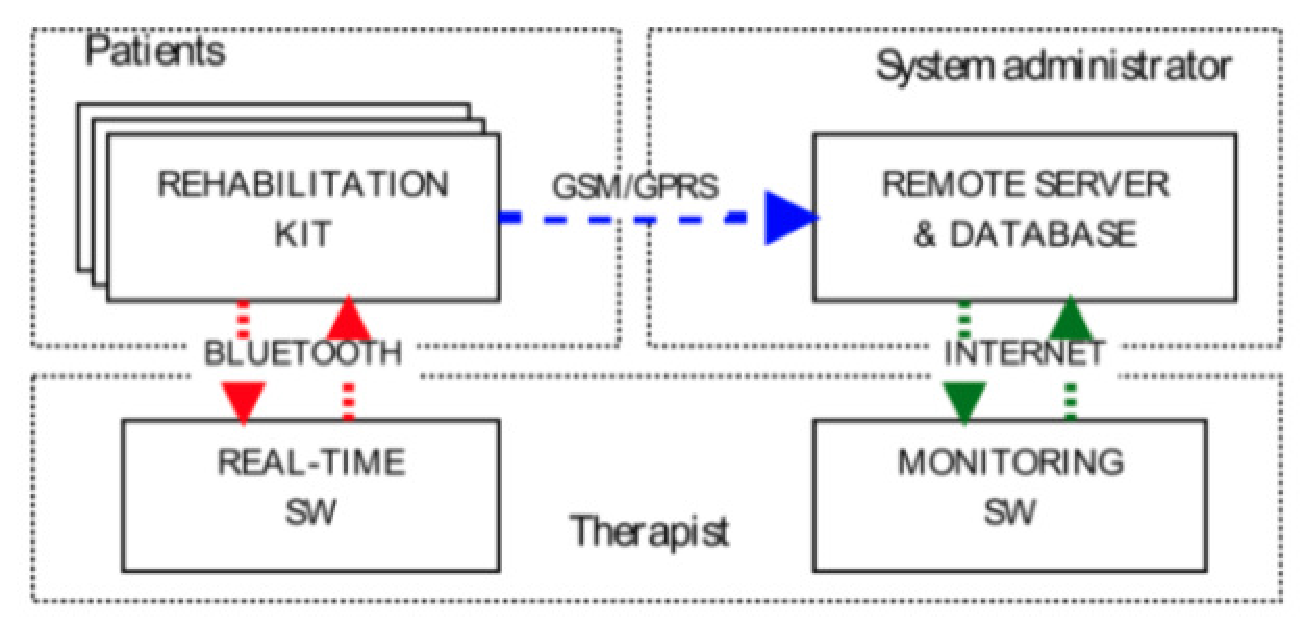
\includegraphics[width=0.7 \textwidth]{img/cap3/pani2014-components}
\caption{Main components of the tele monitoring system \cite{pani2014}}
\label{fig:pani2014-components}
\end{center}
\end{figure}

The rehabilitation kit presented suggests an interesting approach when the assembly of specific hardware is needed and when there is no Internet to do data transfer. The use of an intermediate server to provide the therapist with access to offline statistical data can be extended to other applications, such as PW users rehabilitation. On the telemonitoring system, only statistical data (related to user's performance during exercise execution) is collected for the therapist. 

In this telerehabilitation tool, the video streaming showing the execution of the exercises is also important, even with the network traffic overhead. Then, the therapist can assess if each set of exercises has been rightly  performed by the user, increasing the efficiency of treatment. 


\subsection{Development of Remote Controllable Visiting Robot}
\label{subsec:mitsumura2014}

Due to the depopulation and ageing across the location, the number of wheelchair users has raised. The family or caregiver cannot  easily go to see him or her, because it takes a lot of time and is costly \cite{mitsumura2014}. 

The work proposed by Mitsumura et al. \cite{mitsumura2014} shows a remote-controlled wheelchair robot development, to be driven safely by a remote user with the function of telepresence and shared with family members or caregivers. The system functions and components are respectively represented in Figures \ref{subfig:mitsumuraSolutions} and \ref{subfig:mitsumuraArchitecture}. 

\begin{figure}[!htbp]
\center
\begin{minipage}{0.495\linewidth}
\center
\captionsetup{justification=centering,margin=0.5cm,font=small}
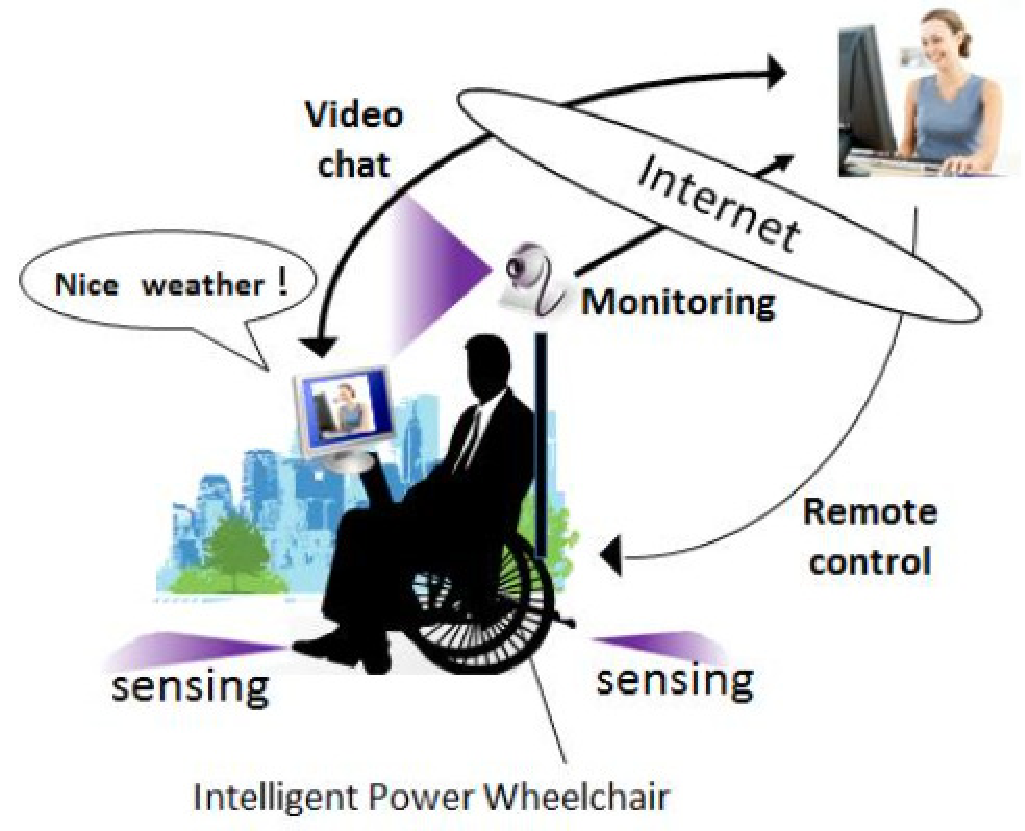
\includegraphics[width=0.8\linewidth]{img/cap3/mitsumuraSolutions}
\caption{ Image of this robot system \cite{mitsumura2014} } \label{subfig:mitsumuraSolutions}
\end{minipage}
\begin{minipage}{0.495\linewidth}
\center
\captionsetup{justification=centering,margin=0cm,font=small}
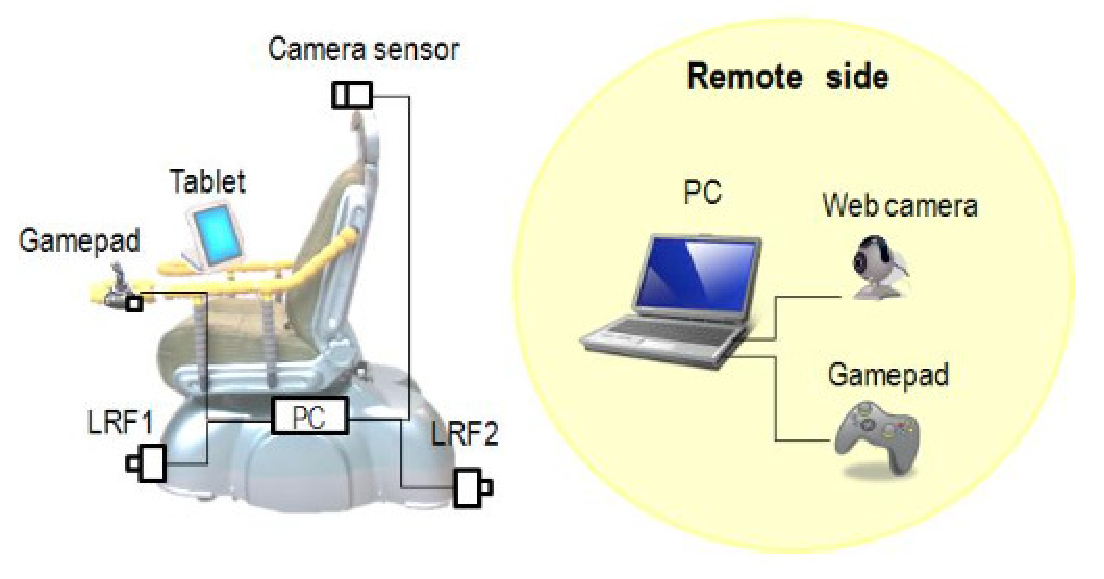
\includegraphics[width=1\linewidth]{img/cap3/mitsumuraArchitecture}
\caption{System architecture components \cite{mitsumura2014} } \label{subfig:mitsumuraArchitecture}
\end{minipage}
\end{figure}


To establish visual communication between the environments, the Skype\texttrademark \hspace{3pt}program was used. The Robot Service Network Protocol (RSNP) was also used to allow the remote control and the function of remote monitor on the base. RSNP is the communication protocol for robot service using Internet, which has been developed by Robot Service Initiative (RSI)\nomenclature{RSI}{Robot Service Initiative} \cite{Rsi2020}. The communication infrastructure of RSNP is a web service one. RSNP provides communication function, multimedia function and robot service function as a module.

The robot system was developed based on the Buddy (wheelchair robot) and RT-Middleware, as shown in Figure \ref{subfig:mitsumuraArchitecture}.

\begin{figure}[!htbp]
\center
\begin{minipage}{0.495\linewidth}
\center
\captionsetup{justification=centering,margin=0.5cm,font=small}
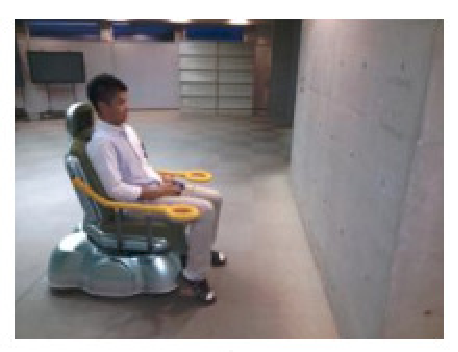
\includegraphics[width=0.9\linewidth]{img/cap3/mitsumuraExperimentsA}
\caption{ Local user control \cite{mitsumura2014}} \label{subfig:mitsumuraExperimentsA}
\end{minipage}
\begin{minipage}{0.495\linewidth}
\center
\captionsetup{justification=centering,margin=0cm,font=small}
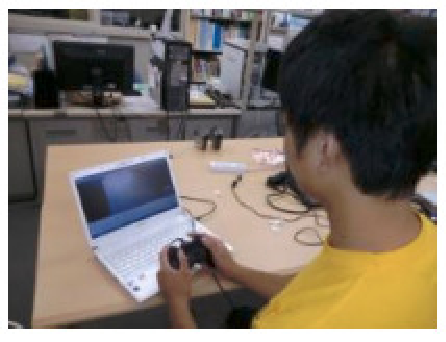
\includegraphics[width=0.86\linewidth]{img/cap3/mitsumuraExperimentsB}
\caption{Remote user control \cite{mitsumura2014}} \label{subfig:mitsumuraExperimentsB}
\end{minipage}
\end{figure}


In this work, a remote controllable wheelchair with telepresence function has been developed. However, experiments conducted on seven people controlling the wheelchair robot locally and remotely, as shown in Figures \ref{subfig:mitsumuraExperimentsA} and \ref{subfig:mitsumuraExperimentsB}, report that five in seven people felt insecure, while being driven by a remote user than driving by one's own self. The reason was thought to be due to the fear of delay of the remote control and Skype. Indeed, there is a risk of disconnection from the network between remote side and local side. To solve this, a supervisor module was developed to stop the smart wheelchair automatically  at the moment when the network seems to be disconnected. 

From the Mitsumura et al. \cite{mitsumura2014} work, some critical aspects have to be considered when the work boundary is telerehabilitation of PW users. First, the possibility of the therapist remotely intermediate, if were necessary, on the user training. Second, as the Internet link, during the training process, may fall or disconnected temporarily, an emergency stop has to be implemented to avoid a crash on remote PW.  


\subsection{A Mobile Gait Rehabilitation System}
\label{subsec:wei2013}

The mobile gait system is composed of network devices, computers, monitoring sensors, actuators, running embedded controls and decision making algorithms, as shown in Figure \ref{fig:wei2013-mobileGaitOverview}. The devices responsible for capturing the user's movements are linked to motion sensors and smart shoes. Mobile robots are used to provide assistive torque to the user's knee joint. The system also allows the therapist to remotely control user's exercises.

\begin{figure}[!hbt]
\begin{center}
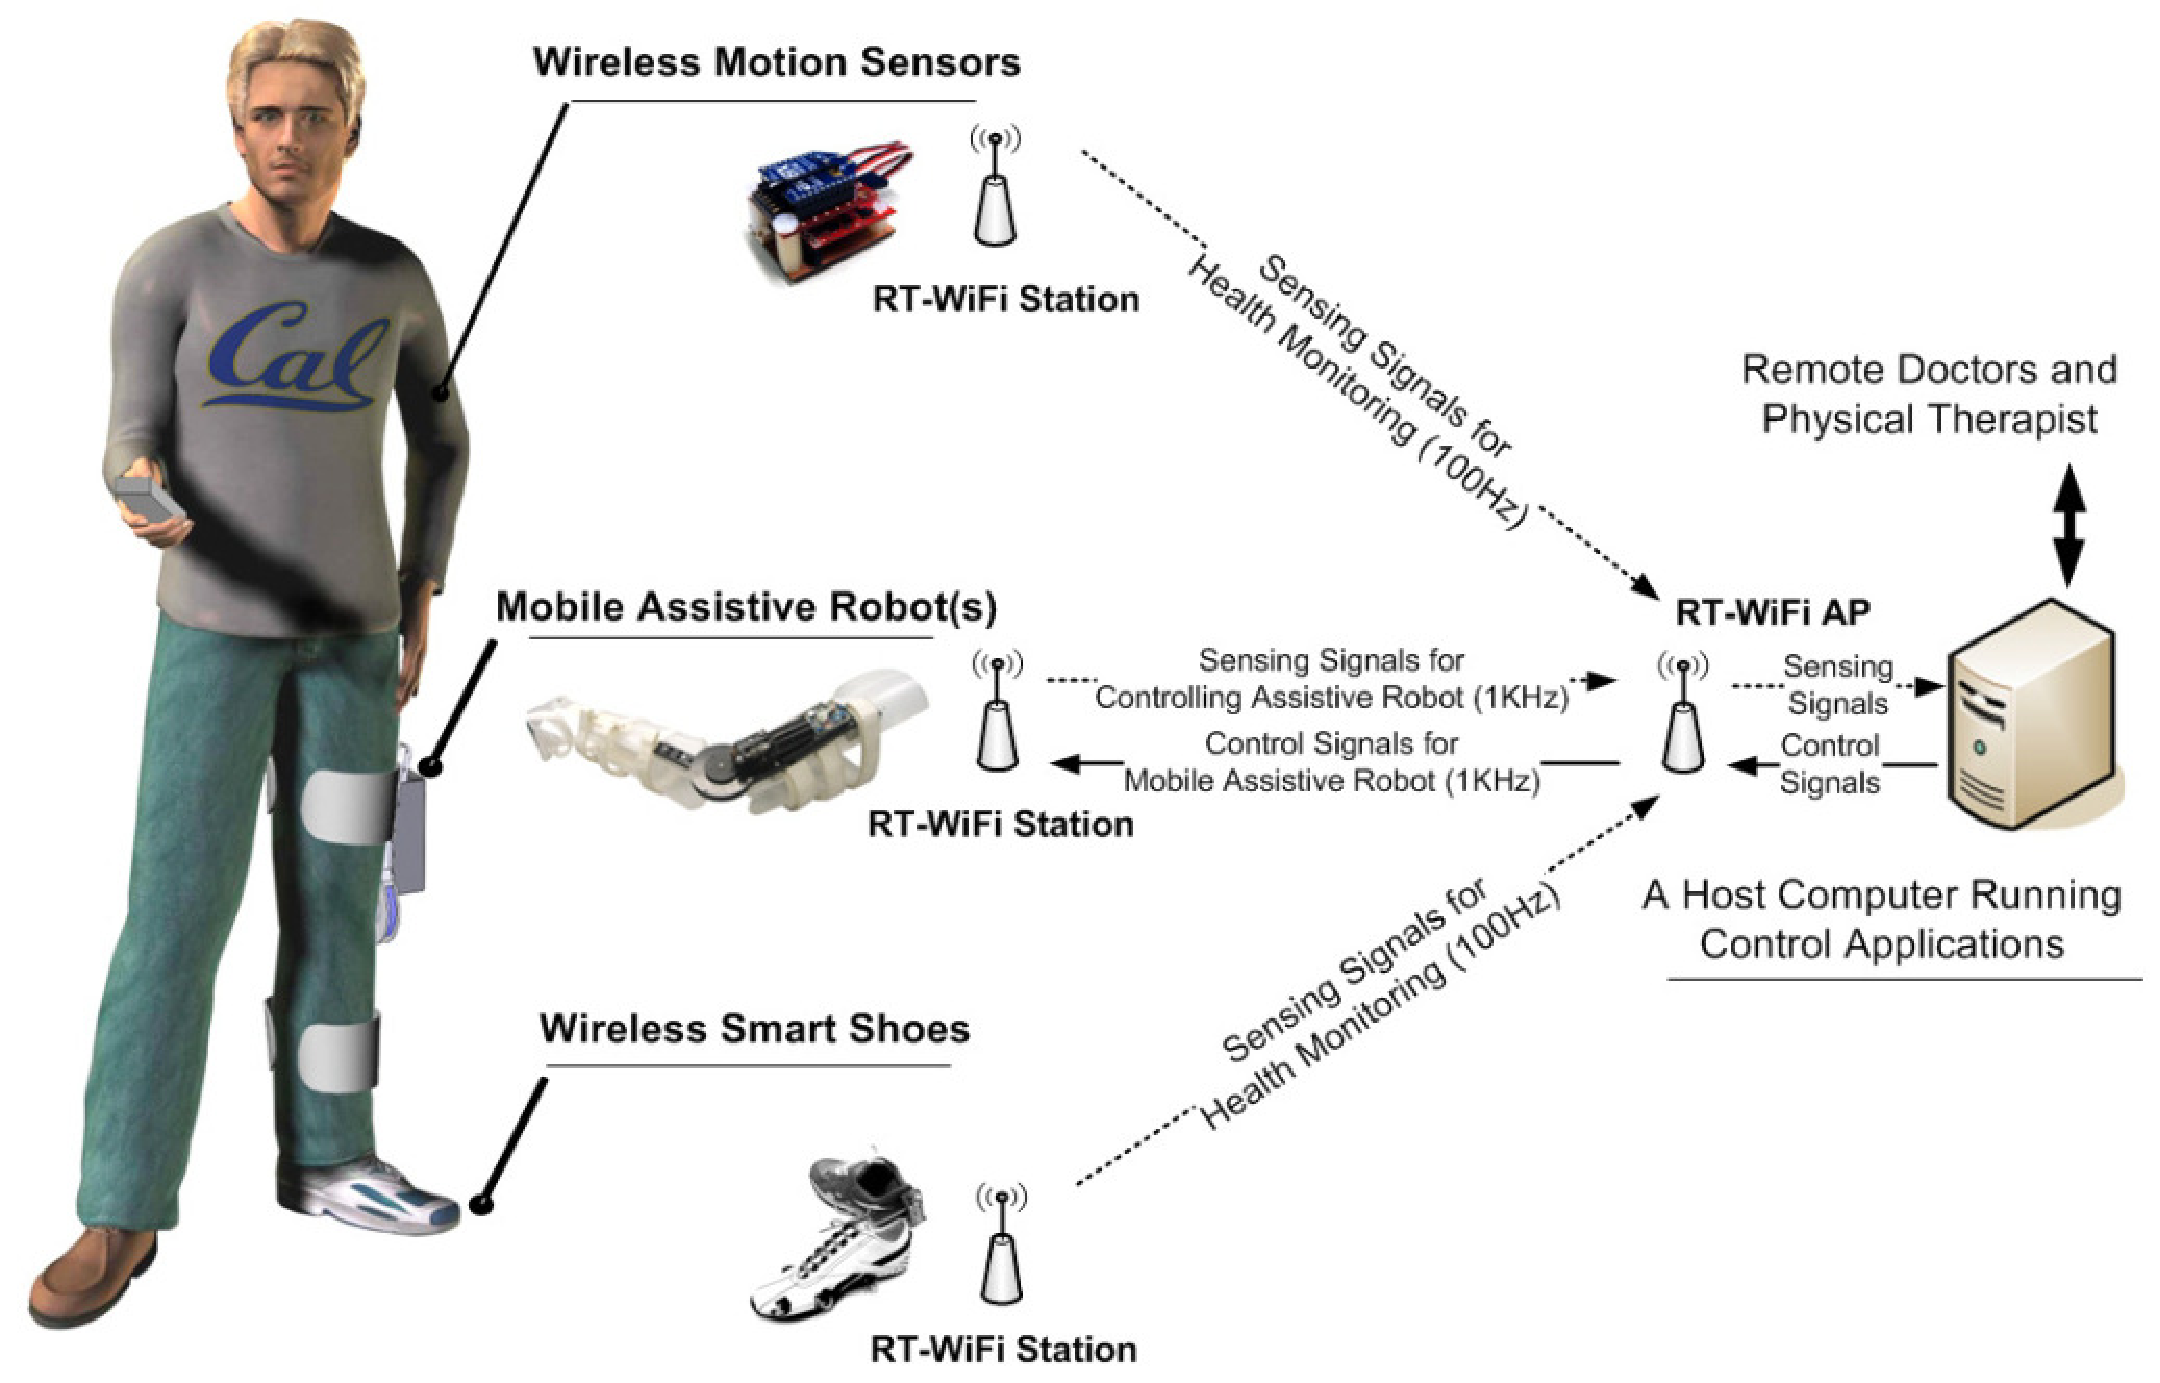
\includegraphics[width=0.9 \textwidth]{img/cap3/wei2013-mobileGaitOverview}
\caption{Overview of the mobile gait rehabilitation system \cite{wei2013}}
\label{fig:wei2013-mobileGaitOverview}
\end{center}
\end{figure}

Real-Time WiFi (RT-WiFi) network protocol serves as the wireless communication subsystem between control application and the rehabilitation device for improved system mobility and telerehabilitation. 

The RT-WiFi was designed to provide a real-time high-sampling-rate data transmission. The design of RT-WiFi is to provide enough freedom for supporting designers to choose their preferred communication behaviour. At the same time, the design of RT-WiFi should minimise the modification on the original Wi-Fi protocol. It must be transparent to both the upper layer software stack and underlying hardware. For instance, Figure \ref{fig:wei2013-RTWiFibased} presents a system architecture plan to deploy three sensors and three actuators into  this system. Depending of the physical proximity of each sensor/actuator, they are attached to different RT-WiFi stations. On a RT-WiFi network, a network manager and control application are running on top of the RT-WiFi Access Point (AP).

\begin{figure}[!hbt]
\begin{center}
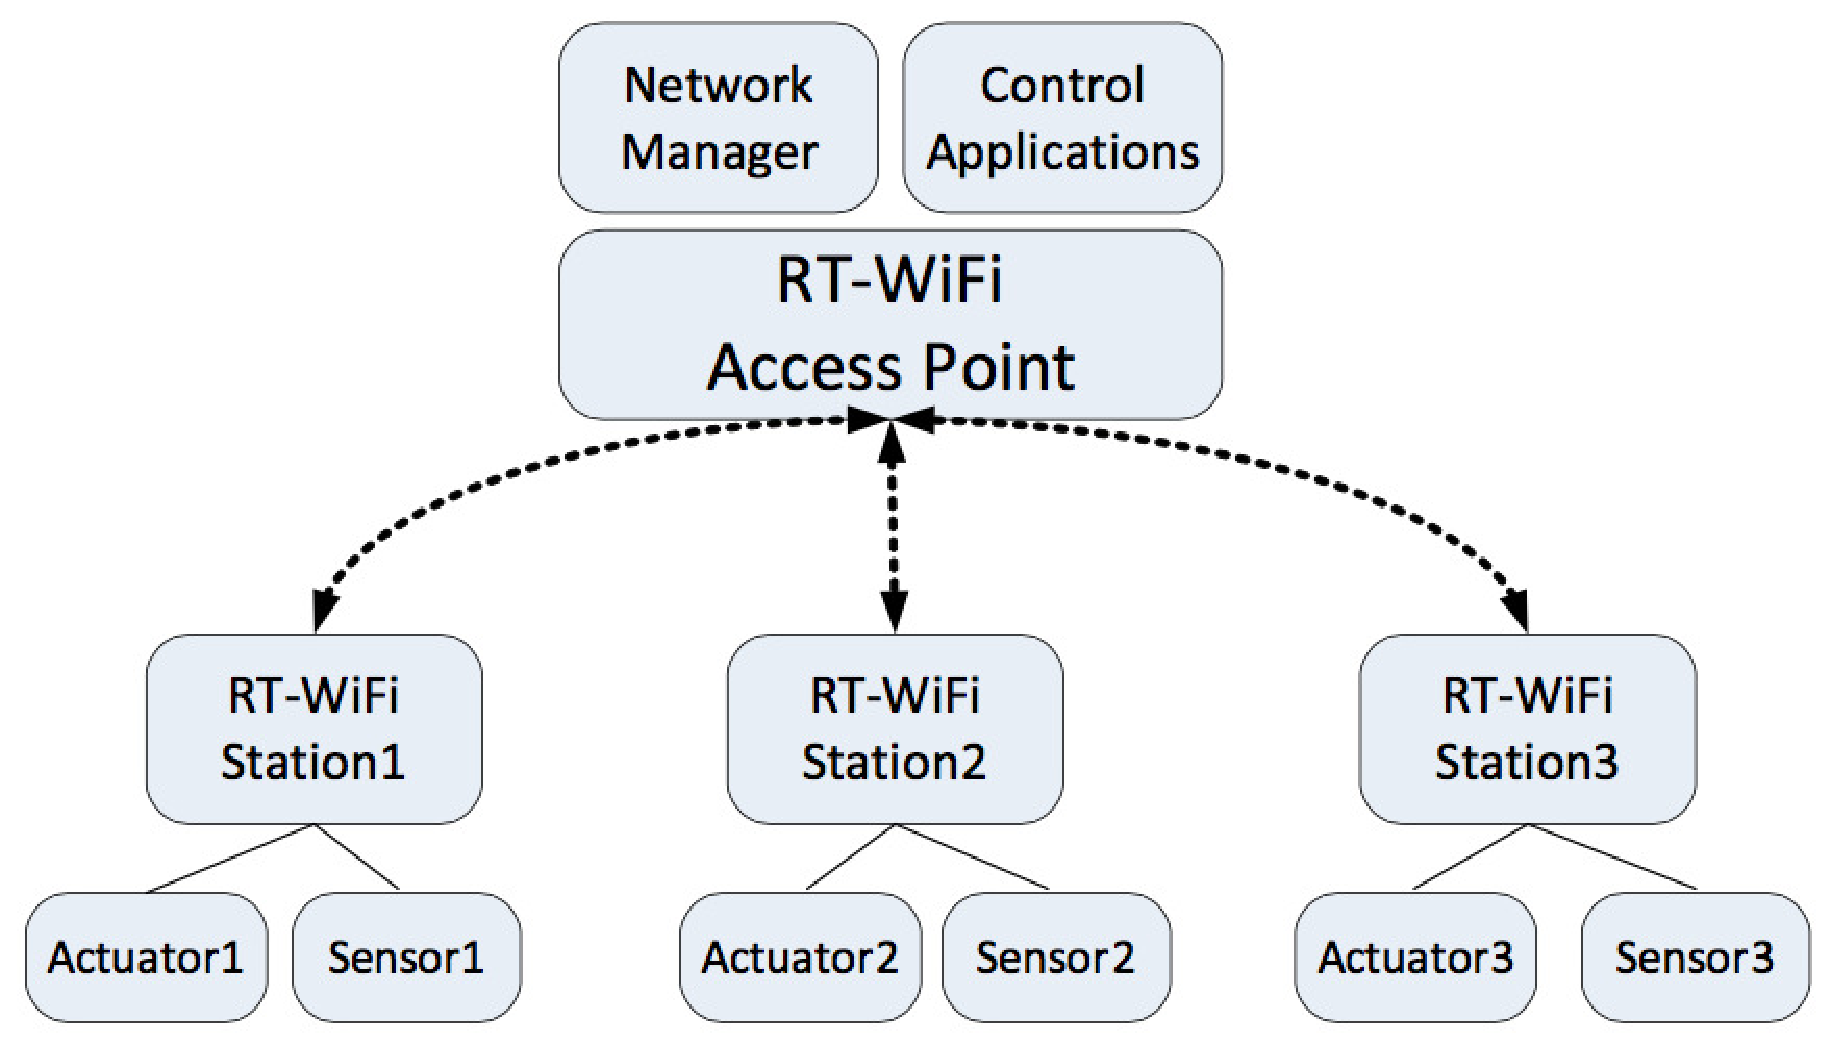
\includegraphics[width=0.7 \textwidth]{img/cap3/wei2013-RTWiFibased}
\caption{RT-WiFi-based wireless control system \cite{wei2013}}
\label{fig:wei2013-RTWiFibased}
\end{center}
\end{figure}

Information time transfer (latency) into Internet applications is a highly important topic in the telerehabilitation and control systems. The presented RT-WiFi protocol is presented as a control paradigm that makes the control interface more efficient and reduces the latency on samples transferred during the process. So, this feature must be considered no matter the system, even for remote wheelchair training, by improving system performance and user experience at the same time. 


\subsection{PerMMA for wheelchair users}
\label{subsec:cooper2012}

The first generation of a Personal Mobility and Manipulation Appliance (PerMMA) for wheelchair users is presented by Cooper et al. \cite{cooper2012}.  PerMMA is a mobile robot as presented in Figure \ref{subfig:cooper2012-robotView}, which has full power seat functions and a custom track system that interfaces with two robotic manipulators. 

\begin{figure}[!htbp]
\center
\begin{minipage}{0.45\linewidth}
\center
\captionsetup{justification=centering,margin=0.5cm,font=small}
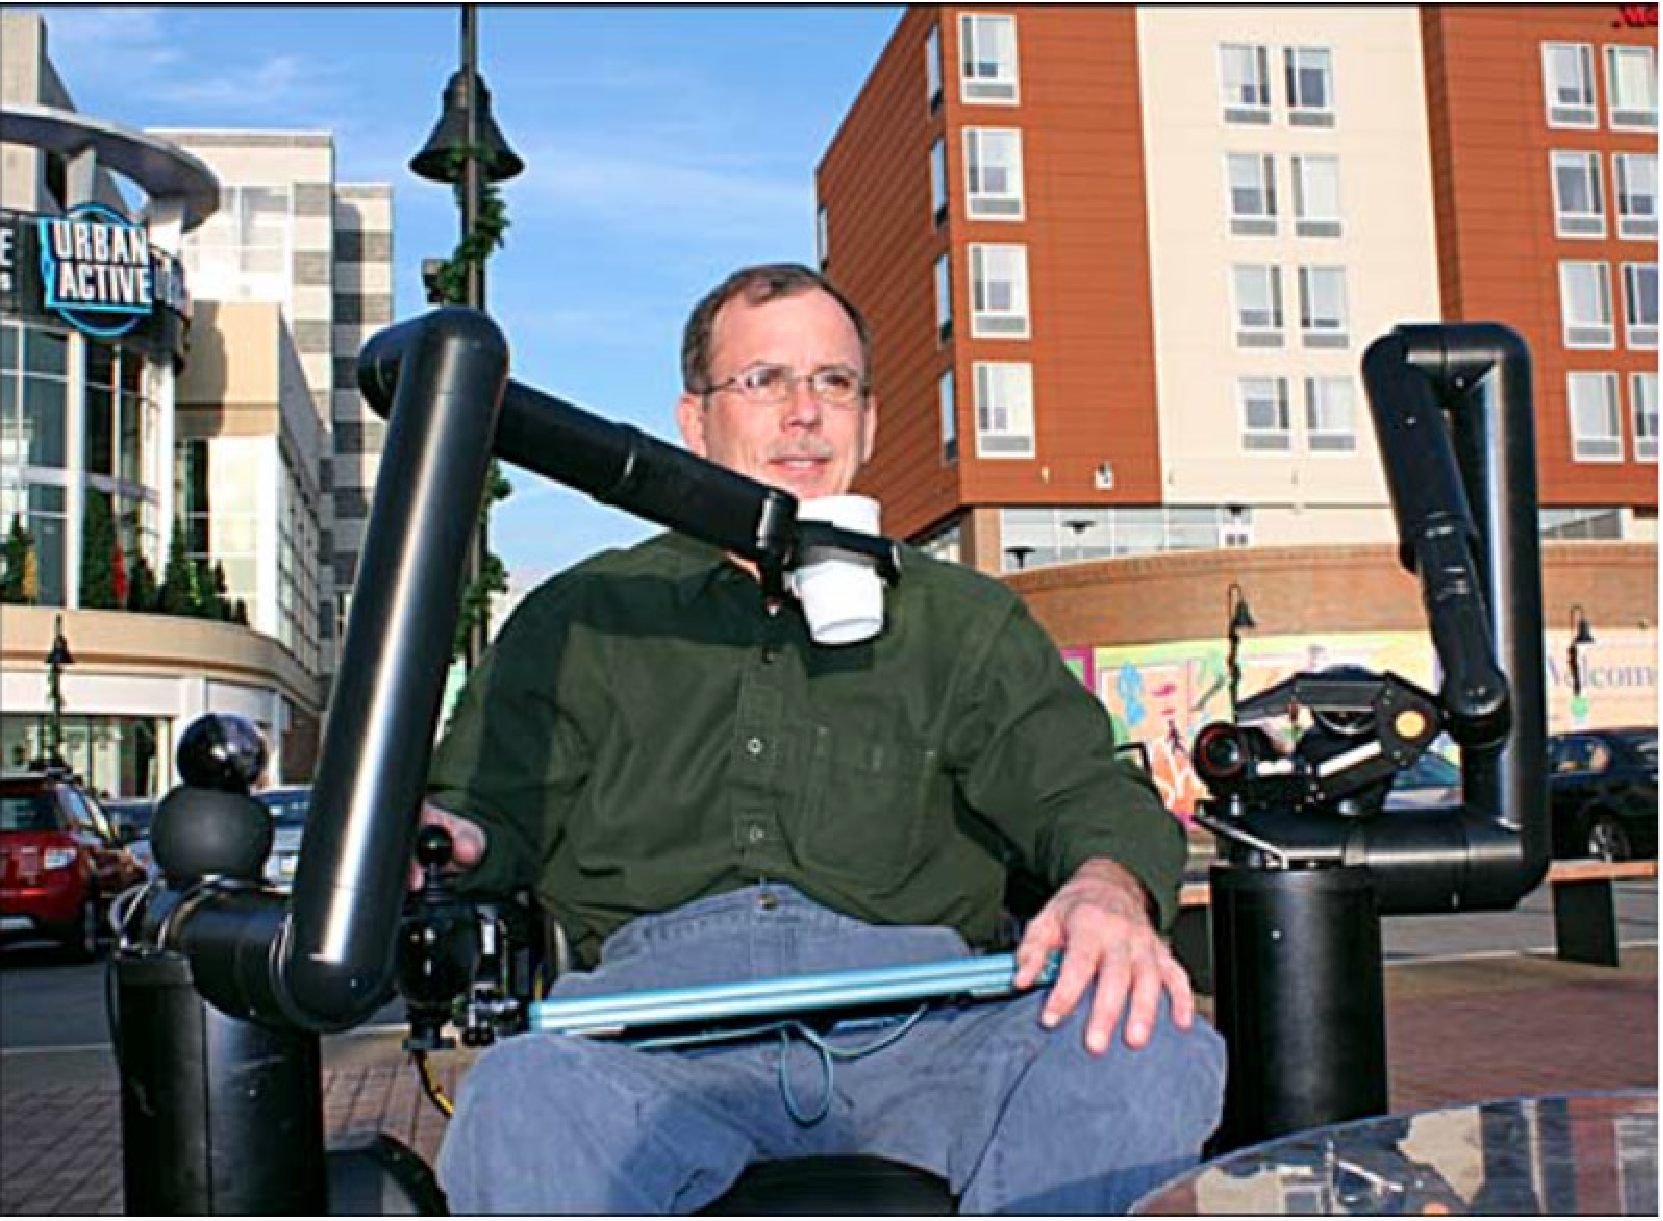
\includegraphics[width=1.1\linewidth]{img/cap3/cooper2012-robotView}
\caption{PerMMA \cite{cooper2012}} \label{subfig:cooper2012-robotView}
\end{minipage}
\begin{minipage}{0.45\linewidth}
\center
\captionsetup{justification=centering,margin=0cm,font=small}
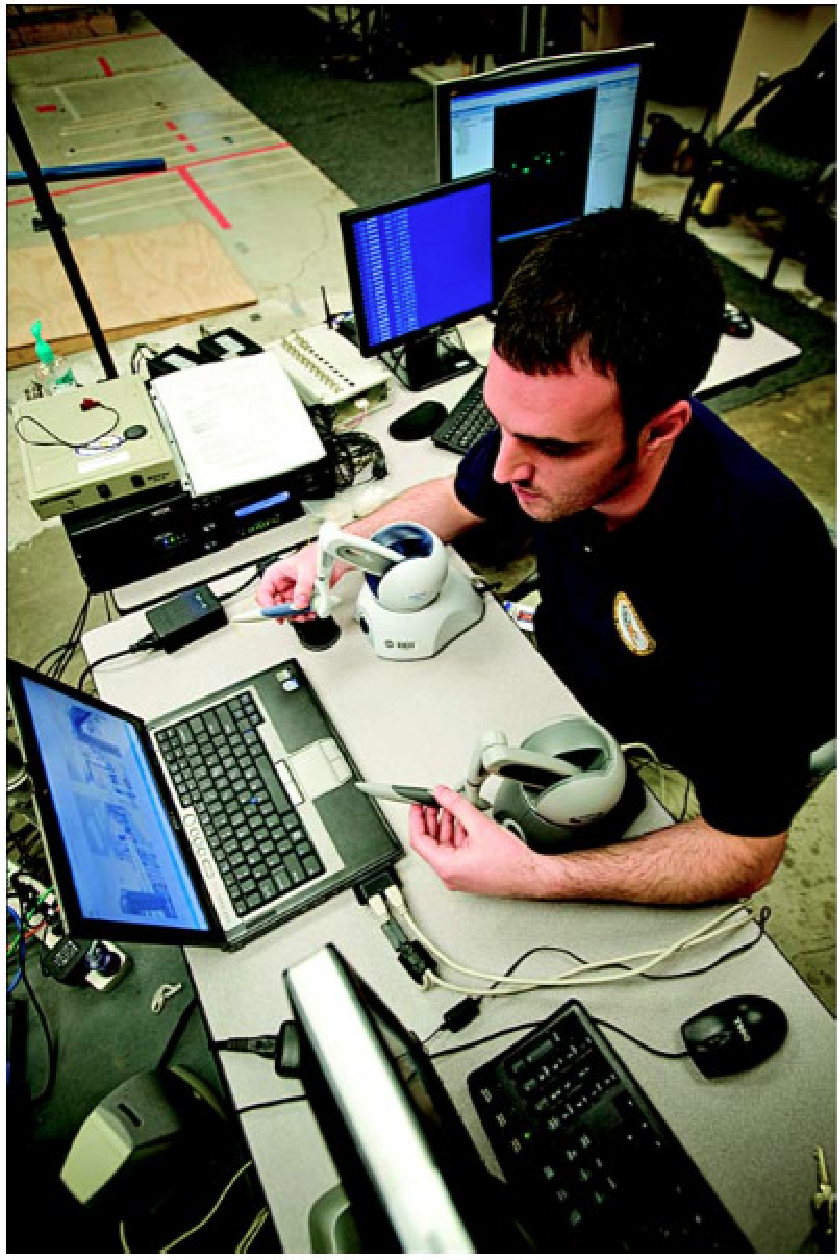
\includegraphics[width=0.7\linewidth]{img/cap3/cooper2012-remoteOp}
\caption{Remote operator station for PerMMA \cite{cooper2012}} \label{subfig:cooper2012-remoteOp}
\end{minipage}
\end{figure}

The control of the PerMMA is maintained by the person in the chair, although control can be shared with a remote assistant at the same time, as presented in Figure \ref{subfig:cooper2012-remoteOp}. It allows a computer view data streaming from the PerMMA and to haptic robots mapped to the arm in the PerMMA. These features allow the user to complete tasks faster when they are not able to finish these task by himself.


The PerMMA is an example of how the knowledge base concerning wheelchair technology has grown. These improvements offer to wheelchair users a better quality of life. However, as stated by the authors, some issues still remain elusive, such as, optimization of wheelchair training and assessment tools. Despite this,  the possibility to remotely assist the user during the training session visually and also interact with a PW become a relevant feature to a telerehabilitation system.

\section{Final Considerations}

The research projects that represent state of the art reveal elements and challenges that have to be considered in an augmented telerehabilitation system to support PW users' training. Telerehabilitation with remote assistance and real-time interaction is a standard feature, as well as, the latency challenge. Besides, media streaming technology is an essential issue for providing visual feedback to the user. And, combined with AR techniques, improves the user experience and also allows meet their needs individually. AR techniques also allow the therapist to customize the session objects. Finally, reliable and standard assessment methodologies are another important subject. All these elements will be further investigated in this research. 


\begin{table}[!hbt]
\centering
\caption{Comparative summary of related work}
\begin{tabular}{ >{\centering}m{8cm} | >{\centering}m{1cm} | >{\centering}m{1cm} | >{\centering}m{1.1cm} | >{\centering}m{1cm} }
\hline
\cellcolor[gray]{0.9} \textbf{Related Work} & 
\cellcolor[gray]{0.9} \begin{sideways} \textbf{Telerehabilitation} { }\end{sideways}&
\cellcolor[gray]{0.9} \begin{sideways} \textbf{PW training} \end{sideways}&
\cellcolor[gray]{0.9} \begin{sideways} \parbox{4.5cm}{\textbf{\hspace{5pt}Training assessment}}{ } \end{sideways}& 
\cellcolor[gray]{0.9} \begin{sideways} \textbf{\hspace{-20pt}AR} \end{sideways}

\tabularnewline\hline \cite{abdallah2019}  	&  \vspace{2.5pt}\no    & \vspace{2.5pt}\no  & \vspace{2.5pt}\no   & \vspace{2.5pt}\yes  
\tabularnewline\hline \cite{vailland2019}  	&  \vspace{2.5pt}\no    & \vspace{2.5pt}\yes  & \vspace{2.5pt}\no   & \vspace{2.5pt}\no  
\tabularnewline\hline \cite{valentini2019}  	&  \vspace{2.5pt}\no    & \vspace{2.5pt}\yes  & \vspace{2.5pt}\yes   & \vspace{2.5pt}\no   
\tabularnewline\hline \cite{borresen2019} 	&  \vspace{2.5pt}\yes    & \vspace{2.5pt}\no  & \vspace{2.5pt}\no   & \vspace{2.5pt}\yes   
\tabularnewline\hline \cite{zolotas2018}  	&  \vspace{2.5pt}\no    & \vspace{2.5pt}\no  & \vspace{2.5pt}\no    & \vspace{2.5pt}\yes  
\tabularnewline\hline \cite{john2018}  		&  \vspace{2.5pt}\no    & \vspace{2.5pt}\yes  & \vspace{2.5pt}\yes   & \vspace{2.5pt}\no   
\tabularnewline\hline \cite{macgillivray2018}  	&  \vspace{2.5pt}\no    & \vspace{2.5pt}\yes  & \vspace{2.5pt}\yes   & \vspace{2.5pt}\no   
\tabularnewline\hline \cite{affanni2018}  	&  \vspace{2.5pt}\no    & \vspace{2.5pt}\yes  & \vspace{2.5pt}\yes   & \vspace{2.5pt}\no   
\tabularnewline\hline \cite{maule2017}  		&  \vspace{2.5pt}\no    & \vspace{2.5pt}\no  & \vspace{2.5pt}\no   & \vspace{2.5pt}\yes   
\tabularnewline\hline \cite{kamaraj2016}     	&  \vspace{2.5pt}\no    & \vspace{2.5pt}\yes  & \vspace{2.5pt}\yes   & \vspace{2.5pt}\no   
\tabularnewline\hline \cite{mitsumura2014}       &  \vspace{2.5pt}\yes    & \vspace{2.5pt}\no  & \vspace{2.5pt}\no   & \vspace{2.5pt}\no   
\tabularnewline\hline \cite{pani2014}       &  \vspace{2.5pt}\yes    & \vspace{2.5pt}\no  & \vspace{2.5pt}\no    & \vspace{2.5pt}\no   
\tabularnewline\hline \cite{wei2013}        	&  \vspace{2.5pt}\yes    & \vspace{2.5pt}\no  & \vspace{2.5pt}\no   & \vspace{2.5pt}\no    
\tabularnewline\hline \cite{cooper2012}     	&  \vspace{2.5pt}\yes    & \vspace{2.5pt}\no  & \vspace{2.5pt}\no   &  \vspace{2.5pt}\no
%\tabularnewline\hline \cite{caetano2020}     	&  \vspace{2pt}\yes    & \vspace{2pt}\yes  & \vspace{2pt}\yes   & \vspace{2pt}\yes 
\tabularnewline\hline
\end{tabular}
\label{tab:relacionado1}
\end{table}


Table \ref{tab:relacionado1} presents a summary of the related work described in this chapter, considering the following features:
\begin{itemize}
\item \textit{Telerehabilitation}: applications where users and therapists are located in different environments;
\item \textit{PW Training}: computer-assisted training of wheelchair users;
\item \textit{Training Assessment}: reliable and standard assessment methodology and procedures to be applied after training sessions; and
\item \textit{AR}: use of AR in health applications increase user experience with real world and also allows the therapist customize the training environment with different virtual objects and positions.
\end{itemize}


By analyzing Table \ref{tab:relacionado1}, it is possible to note that until the present moment, a system with all features above, has not been found in the literature. It's believed that through these features, the user and therapist will be connected to a training environment and interacting in a more natural, secure, and efficient way. The idea is to have a user who, from any place with Internet and a computer, will issue commands necessary to control a PW and, at the same time, will receive visual augmented feedback in a traditional monitor device. Each user has different impairments and thus the therapist can set up a specific amount of tasks that will make part of the training protocol.  Therefore, this research proposes the investigation of computer techniques that support the integration of all these features.

In the next chapter, the materials and methods used in this research will be detailed, as well as the proposed solution components.

